\input{../title}

\chapter{Introduction}

The following background on building energy modeling (BEM) will provide
a foundation before learning the essentials of EnergyPlus. If you
are already familiar with BEM, you may wish to skip to Section 1.4
describing the EnergyPlus QuickStart Guide.

\section{What is BEM?}

According to the \href{https://www.bemlibrary.com/index.php/owners-managers/introduction/what-bem/}{BEM Library}:
\begin{quotation}
``Building Energy Modeling (BEM) is the practice of using computer-based
simulation software to perform a detailed analysis of a building\textquoteright s
energy use and energy-using systems. The simulation software works
by enacting a mathematical model that provides an approximate representation
of the building. BEM includes whole-building simulation as well as
detailed component analysis utilizing specialized software tools that
address specific concerns, such as moisture transfer through building
materials, daylighting, indoor air quality, natural ventilation, and
occupant comfort. BEM offers an alternative approach that encourages
customized, integrated design solutions, which offer deeper savings.
Using BEM to compare energy-efficiency options directs design decisions
prior to construction. It also guides existing building projects to
optimize operation or explore retrofit opportunities.''
\end{quotation}
Some other terms that are used to describe the same topic are:
\begin{itemize}
\item Building Simulation
\item Building Performance Simulation
\item Building Energy Simulation
\item Building Performance Modeling
\end{itemize}
Somewhat confusing, the term ``model'' can refer to both the specific
building being described and analyzed as well as referencing the software
for implementing a specific component of the building such as a wall
or chiller.

To learn more about building energy modeling consider reviewing the
following resources:
\begin{itemize}
\item \href{https://www.ashrae.org/technical-resources/ashrae-handbook/description-2017-ashrae-handbook-fundamentals}{2017 ASHRAE Handbook - Fundamentals }Chapter
19 Energy Estimating and Modeling Methods
\item \href{https://www.bemlibrary.com/}{BEM Libary}
\item \href{http://www.ibpsa.org/?page_id=695}{IBPSA}, \href{https://www.ibpsa.us/videos/all}{IBPSA-USA},
and \href{https://www.youtube.com/results?search_query=building+energy+modeling}{YouTube}
videos
\item \href{https://www.amazon.com/s/ref=nb_sb_noss_2?url=search-alias\%3Daps&field-keywords=building+energy+modeling}{Numerous books}
\item ASHRAE \href{https://www.techstreet.com/ashrae/standards/ashrae-209-2018?gateway_code=ashrae&product_id=2010483}{Standard 209}
Energy Simulation Aided Design for Buildings Except Low-Rise Residential
Buildings
\item Study materials for the ASHRAE Building Energy Modeling Professional
(\href{https://www.ashrae.org/professional-development/ashrae-certification/certification-types/bemp-building-energy-modeling-professional-certification}{BEMP})
or AEE Building Energy Simulation Analyst (\href{https://www.aeecenter.org/certifications/certifications/certified-building-energy-simulation-analyst}{BESA})
professional certifications
\end{itemize}
Building energy modeling is necessary to understand the overall energy
consumption in buildings, because, the energy flows in buildings can
be very complicated. The heat flow through walls is determined not
just by the area and the temperatures, but the mass characteristics
of the walls may result in heat flowing out of a wall several hours
after it has flowed in. The constantly changing temperature on the
outside of the wall and the less frequent but often large step changes
in thermostat setpoints between day and night operation for the inside
of the building make the direction of the heat flow vary over time.
Solar energy is absorbed on the exterior wall and roof surfaces as
well as entering windows. The intensity of solar energy varies by
the sun position for each period of time over the day and over the
year. Heat sources within the building including people, office and
other equipment, and lighting include both heat that immediately impacts
the air within (convective heat) and heat that is absorbed by the
surfaces and released slowly over time (radiant heat). Lighting may
be controlled by a sensor that turns it on or off or changes its intensity
based on the amount of natural daylight that is entering the space
through windows and skylights making the heat generated from the lighting
system change over time. Air conditioning and heating systems come
in a huge number of configurations, and each one can be used with
many different control configurations based on the temperature or
other conditions within each space in the building, and ultimately
their operation accounts for a large portion of the energy consumed
in a building. For these reasons and more, what might first appear
as something that can be calculated with just a few formulas in a
spreadsheet is instead a software program and, in the case of EnergyPlus,
with over 500,000 lines of code.

\section{Questions that BEM can answer}

The most common questions that BEM can answer are:
\begin{itemize}
\item If my building was made or operated differently, how would the required
equpment capacity and energy consumption change?
\item Does my building comply with a building energy code or standard?
\item What kind of rating or how many points can I get in an environmental
certification program?
\item Is my building operating as it was designed to?
\item What is a good target for energy consumption for my building?
\end{itemize}
These questions and more can occur at different times during the life-cycle
of a building, from before schematic design all the way through the
rest of the design process, and into the operation of the building

\section{The Design Process and BEM }

Building energy modeling can be used throughout the design process
for a new building or when considering updates to existing buildings.
It can also be used later in the life-cycle of a building related
to comparing actual operation of the building with the predicted operation.
ASHRAE \href{https://www.techstreet.com/ashrae/standards/ashrae-209-2018?gateway_code=ashrae&product_id=2010483}{Standard 209}
titled ``Energy Simulation Aided Design for Buildings Except Low-Rise
Residential Buildings'' is a critical document in how to apply building
energy modeling. It describes a methodology to apply building energy
modeling to the design and was created to define reliable and consistent
procedures that advance the use of timely energy modeling to quantify
the impact of design decisions at the point in time which they are
made. The standard includes different \textquotedblleft Modeling Cycles\textquotedblright{}
for different stages of using building energy modeling during the
life-cycle of the building:
\begin{itemize}
\item Modeling Cycle \#1 -- Simple Box Modeling
\item Modeling Cycle \#2 -- Conceptual Design Modeling
\item Modeling Cycle \#3 -- Load Reduction Modeling
\item Modeling Cycle \#4 -- HVAC System Selection Modeling
\item Modeling Cycle \#5 -- Design Refinement
\item Modeling Cycle \#6 -- Design Integration and Optimization
\item Modeling Cycle \#7 -- Energy Simulated-Aided Value Engineering
\item Modeling Cycle \#8 -- As-Designed Energy Performance
\item Modeling Cycle \#9 -- Change Orders
\item Modeling Cycle \#10 -- As-Built Energy Performance
\item Modeling Cycle \#11 -- Postoccupancy Energy Comparison
\end{itemize}
In addition, it has information about how to integrate climate and
site analysis, benchmarking, energy charrettes (a meeting of the stakeholders
to discuss goals and design strategies) and the energy performance
goals of the owners project requirements into the design process when
using building energy modeling.

\section{EnergyPlus QuickStart Guide}

Don't be intimidated by the apparent complexity of EnergyPlus; you
can get started using EnergyPlus quickly using the QuickStart Guide
which is part of the documentation. It shows you how you can use just
an input file and some output files to start seeing results quickly.
The building description, the detecting and solving of errors, and
the most common primary outputs are found in the IDF input file, the
Table.HTML output file and the .ERR diagnostics file. Starting with
these three files and branching out to others as needed is a good
strategy for learning EnergyPlus.

\section{EnergyPlus Capabilities}

According to the \href{https://energyplus.net/}{energyplus.net web site}
(as of January 2019):
\begin{quotation}
``EnergyPlus\texttrademark{} is a whole building energy simulation
program that engineers, architects, and researchers use to model both
energy consumption---for heating, cooling, ventilation, lighting
and plug and process loads---and water use in buildings. Some of
the notable features and capabilities of EnergyPlus include:
\end{quotation}
\begin{itemize}
\item Integrated, simultaneous solution of thermal zone conditions and HVAC
system response that does not assume that the HVAC system can meet
zone loads and can simulate un-conditioned and under-conditioned spaces.
\item Heat balance-based solution of radiant and convective effects that
produce surface temperatures, thermal comfort, and condensation calculations.
\item Sub-hourly, user-definable time steps for interaction between thermal
zones and the environment; with automatically varied time steps for
interactions between thermal zones and HVAC systems. These allow EnergyPlus
to model systems with fast dynamics while also trading off simulation
speed for precision.
\item Combined heat and mass transfer model that accounts for air movement
between zones.
\item Advanced fenestration models including controllable window blinds,
electrochromic glazings, and layer-by-layer heat balances that calculate
solar energy absorbed by window panes.
\item Illuminance and glare calculations for reporting visual comfort and
driving lighting controls.
\item Component-based HVAC that supports both standard and novel system
configurations.
\item A large number of built-in HVAC and lighting control strategies and
an extensible runtime scripting system for user-defined control.
\item Functional Mockup Interface import and export for co-simulation with
other engines.
\item Standard summary and detailed output reports as well as user definable
reports with selectable time-resolution from annual to sub-hourly,
all with energy source multipliers.''
\end{itemize}
In addition:
\begin{itemize}
\item ASCII text-based weather, input, and output files that include hourly
or sub-hourly environmental conditions, and standard and user definable
reports, respectively.
\item Transient heat conduction through building elements such as walls,
roofs, floors, etc. using conduction transfer functions.
\item Thermal comfort models based on activity, inside dry-bulb temperature,
humidity, etc.
\item Anisotropic sky model for improved calculation of diffuse solar on
tilted surfaces.
\item Atmospheric pollution calculations that predict CO2, SOx, NOx, CO,
particulate matter, and hydrocarbon production for both on-site and
remote energy conversion.
\item EnergyPlus can be used for for building load calculations and sizing
equipment and uses the heat balance method recommended in the \href{https://www.ashrae.org/technical-resources/ashrae-handbook}{ASHRAE Handbook Fundamentals}.
Proper sizing of equipment without oversizing, generally saves energy
as the equipment is operated nearer to optimal loads.
\item EnergyPlus runs on Windows, MacOS, and Linux computers.
\end{itemize}
Integration of Loads, Systems, and Plants: One of the strong points
of EnergyPlus is the integration of all aspects of the simulation---loads,
systems, and plants. System and plant output are allowed to directly
impact the building thermal response rather than calculating all loads
first, then simulating systems and plants. The simulation is coupled
allowing the designer to more accurately investigate the effect of
undersizing fans and equipment and what impact that might have on
the thermal comfort of occupants within the building.

\section{Open Source}

\href{https://energyplus.net/}{EnergyPlus} is an \href{https://opensource.org/}{Open Source}
program so all the \href{https://github.com/NREL/EnergyPlus}{source code}
is available to inspect and modify. If you are interested in how calculations
are performed and the \href{https://energyplus.net/documentation}{Engineering Reference}
does not provide enough details to you, you can review the source
code itself. \href{https://github.com/NREL/EnergyPlus/wiki/BuildingEnergyPlus}{Instructions to build the code}
(compile the source code into an executable application) are available
in the source code repository wiki if you see something that needs
to be enhanced or fixed, please also see the \href{https://energyplus.net/contributing}{contribution policy}.

\section{Brief History}

EnergyPlus has been under development since 1997 and was first released
in 2001. EnergyPlus has its roots in both the BLAST and DOE--2 programs.
BLAST (Building Loads Analysis and System Thermodynamics) and DOE--2
were both developed and released in the late 1970s and early 1980s
as energy and load simulation tools. BLAST was developed by the \href{https://www.erdc.usace.army.mil/Locations/CERL/}{Construction Engineering Research Laboratory (CERL)}
and \href{https://illinois.edu/}{the University of Illinois} while
DOE-2 was developed by \href{https://www.lbl.gov/}{Berkeley Lab}
and many others. Their intended audience is a design engineer or architect
that wishes to size appropriate HVAC equipment, develop retrofit studies
for life cycling cost analyses, optimize energy performance, etc.
Born out of concerns driven by the energy crisis of the early 1970s
and recognition that building energy consumption is a major component
of the American energy usage statistics, the two programs attempted
to solve the same problem from two slightly different perspectives.
In the late 1990s, concern about limitations of both BLAST and DOE-2
as well as difficulty in maintaining the old code bases prompted combining
the development efforts for a new program called EnergyPlus. EnergyPlus
was originally written in Fortran, in 2014 it was converted to C++.
It was developed as a simulation engine, and many \href{https://www.buildingenergysoftwaretools.com/}{graphical user interfaces}
utilize it.

\section{Documentation}

The EnergyPlus documentation is currently included in the installation
in the ``Documentation'' folder as PDFs. It is also available as
\href{https://energyplus.net/documentation}{PDFs online} and from
third parties that have generated HTML documentation from the source.
Using search in the documentation is critical to finding the information
needed. Some of the documentation PDFs are very large, so searching
is a good way to find specific information about a topic or an input
object. The documentation includes:
\begin{itemize}
\item QuickStart Guide: Contains a brief high-level overview of EnergyPlus
and get you up and running quickly with the program
\item Input Output Reference: Contains a thorough description of the various
input and output files related to EnergyPlus, the format of these
files, and how the files interact and interrelate.
\item Output Details and Examples: Contains details on output from EnergyPlus.
It also addresses the reference data sets that are included.
\item Auxiliary Programs:~Contains information for the auxiliary programs
that are part of the EnergyPlus package. For example, this document
contains the user manual for the Weather Converter program, descriptions
on using Ground Heat Transfer auxiliary programs with EnergyPlus,
and other assorted topics.
\item Engineering Reference: Provides more in-depth knowledge into the theoretical
basis behind the various calculations contained in the program including
algorithm descriptions.
\item Application Guide for EMS: Provides an in-depth look at the Energy
Management System (EMS) feature which provides a way to develop custom
control and modeling routines.
\item External Interface(s) Application Guide: Contains information specific
to using the external interface feature of EnergyPlus to connect other
simulation systems.
\item Plant Application Guide: Details the methods for simulating chilled
and hot water plant systems within EnergyPlus.
\item Using EnergyPlus for Compliance Guide: Contains information specific
to using EnergyPlus in compliance and standard rating systems.
\item Tips \& Tricks for Using EnergyPlus: Contains short tips and tricks
for using various parts of EnergyPlus.
\end{itemize}

\section{Example Files }

Many hundreds of example files come with EnergyPlus, and they are
in the ExampleFiles folder from the installation. The \textbackslash ExampleFiles\textbackslash ExampleFiles.html
lists each one and includes the name, a description (scroll all the
way to the right) and lots of information such as the floor area and
whether certain types of input objects are included in the file. Often
searching through this file is a good way to find the proper example
file to learn about a feature. Another method is the \textbackslash ExampleFiles\textbackslash ExampleFiles-ObjectsLink.html
file which lists every type of input object that EnergyPlus uses and
then the first three files that use that input object. It is possible
that many other files also use a particular input object so if the
first three files do not help, a text search of files in the ExampleFiles
folder may find more.

\chapter{The EnergyPlus Ecosystem }

\section{Current Interfaces }

EnergyPlus is often used directly using the text file input (IDF or
epJSON) and various output file formats along with the utilities that
come with the installation package. More information on that can be
found in section \ref{sec:Using-EnergyPlus}. In addition, EnergyPlus is often
the simulation engine for graphical user interfaces. To see a list,
see the \href{https://www.buildingenergysoftwaretools.com/}{BEST (Building Energy Software Tools) Directory}
that is operated by \href{https://www.ibpsa.us/}{IBPSA-USA}.

\section{Approaches to Implement Measures }

In the terminology used within the building energy modeling industry
``measures,'' sometimes called energy conservation measures (ECMs)
or energy efficiency measures (EEMs), are when alternative configurations
of a building are considered and simulated and compared with the original
building model. Measures include added wall or roof insulation, lower
internal lighting power, higher efficiency heating and cooling equipment,
and many others. When using EnergyPlus within a graphical user interface,
that interface often provides a way to implement various measures.
When not working within a graphical user interface, users have several
options for implementing measures.

For a specific building input file, a copy of the input file can be
made and then modified to reflect the measure. This is an easy approach
initially, but since the original building model might change, it
means making the change in the file that reflects the measure. When
many measures are being considered, this duplicative editing can be
inefficient and prone to errors. In addition, the measure cannot be
easily applied to a different building energy model without again
editing another set of files duplicating the original effort. Due
to this, it is very common for some type of scripting to be used so
that measures can be applied to the original building model and other
models of other buildings reliably and quickly. Scripting in this
approach means to apply some type of programming language to the task
of modifying files.

EnergyPlus includes, with the installation package, two methods of
implementing measures EP-Macro and the ParametricPreprocessor. EP-Macro
is similar to the C language pre-processor and allows for portions
of the file to be included or excluded, portions of other files to
be included when desired, and for specific entries that are normally
fixed values to change programmatically. EP-Macro is documented in
the AuxiliaryPrograms documentation. A file with lines starting ``\#\#''
or with the ``imf'' file extension is likely to be a file using
EP-Macro commands.

The EnergyPlus ParametricPreprocessor uses special input objects in
EnergyPlus to set values for any field in any other input object for
a series of simple options. This is briefly described in the AuxiliaryPrograms
documentation, and more details are present in the InputOutputReference
under the section on ``Parametric Objects.'' The ParametricPreprocessor
approach is very straight forward, however it has limits in the flexibility
that it provides. It is suitable for implementing measures related
to internal loads, constructions, and simple efficiency changes but
is probably not the appropriate tool for more complicated measures.

A \href{https://www.ashrae.org/File\%20Library/Conferences/Specialty\%20Conferences/2018\%20Building\%20Performance\%20Analysis\%20Conference\%20and\%20SimBuild/Papers/C043.pdf}{paper}
that describes various other approaches to scripting was written during
the 2018 ASHRAE/IBPSA-USA Building Performance Conference and SimBuild.

\section{Parametric Analysis Tools }

When just implementing a simple measure or even a series of measures
is not enough, a parametric analysis tool may be appropriate. These
tools allow the exploration throughout the range of variables (such
as the thickness of insulation in the roof or the efficiency of a
boiler) to see the impacts of optimization. While many of the approaches
used to implement measures described previously may also be used for
parametric analysis, a few specific tools have been developed. To
see a list, see the \href{https://www.buildingenergysoftwaretools.com/}{BEST (Building Energy Software Tools) Directory}
that is operated by \href{https://www.ibpsa.us/}{IBPSA-USA}.

\section{Weather Files \label{subsec:Weather-Files}}

Weather files are available for many locations throughout the world.
Finding the right file that represents the weather in your specific
location can sometimes be a challenge. Often the closest weather location
is the best one to choose, but sometimes a site that is further away
may actually have the most similar weather. This is especially the
case in terrain that varies in elevation or when near large bodies
of water. Many weather files are available from both public and private
sources. The \href{https://energyplus.net/weather}{EnergyPlus weather file }
web site has many weather files with \href{https://energyplus.net/weather/sources}{sources described}.
That web site also has a \href{https://energyplus.net/weather/simulation}{page with links}
to many other sites that provide weather files. The modeler must also
choose between using a typical year weather files or an actual year
file. Typical year files, such as TMY3 and IWEC are representative
of long-term weather compiled from 20-30 years of data. Actual year
files contain a specific year of weather data and generally used for
calibration or verification studies where the simulation results are
compared to actual utility bills or other measured data.

\begin{figure}[hbtp]
\centering
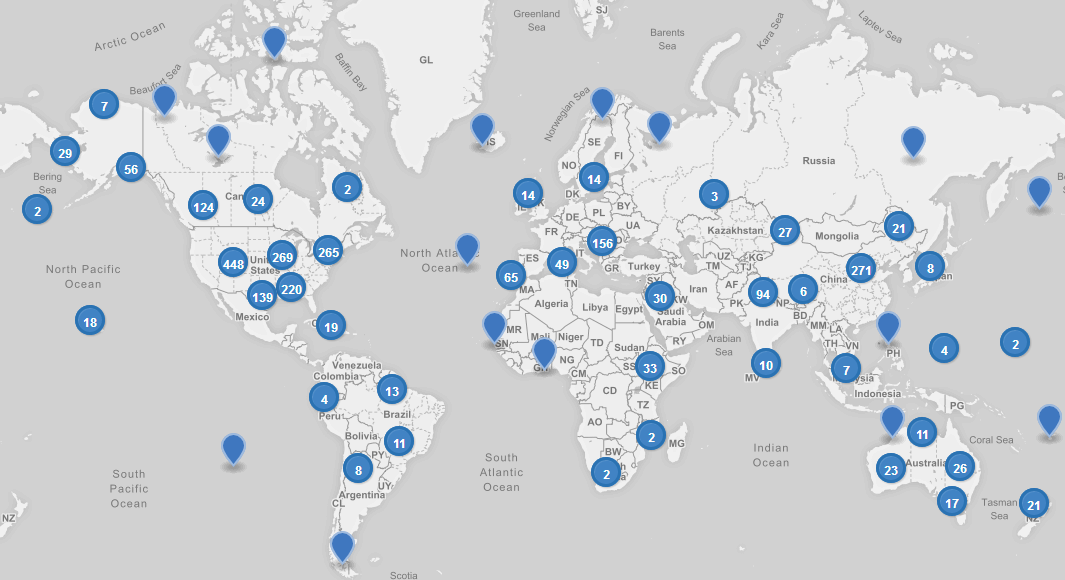
\includegraphics[width=0.9\textwidth, height=0.9\textheight, keepaspectratio=true]{media/WeatherFileLocations.png}
\caption{EnergyPlus.net Weather File Locations}
\end{figure}

\section{Co-Simulation and Linked Software}

The modelling of multi-domain, multi-physics, and multi-time scale
systems such as buildings is a challenge for building energy modelling
and simulation tools. In certain circumstances, it may be better for
modelling such systems to split the systems into multiple sub-systems,
model the individual sub-systems in the language or tool which is
best suited for the system\textquoteright s domain, and use a master
algorithm to link the sub-systems for a so called \textquotedblleft co-simulation.\textquotedblright{}
In a nutshell, co-simulation consists of the theory and techniques
that enable the simulation of a coupled system through the composition
of simulators. Each simulator is an input-output mock-up of a constituent
system, developed and provided by the team that is responsible for
the \href{https://arxiv.org/abs/1702.00686}{sub-system}. The coupling
of the sub-systems is performed by a master algorithm which is responsible
for linking the sub-systems at run-time for data-exchange. EnergyPlus
implements three mechanisms to support co-simulation.
\begin{itemize}
\item EnergyPlus implements the Building Controls Virtual Test Bed ( \href{https://www.tandfonline.com/doi/abs/10.1080/19401493.2010.518631}{BCVTB}) API.
This API leverages the BCVTB to enable the co-simulation of EnergyPlus with various simulation programs such as \href{http://www.trnsys.com/}{TRNSYS},
\href{http://www.esru.strath.ac.uk/Programs/ESP-r.htm}{ESP-r}, \href{http://radsite.lbl.gov/radiance/HOME.html}{Radiance}, or
\href{https://www.3ds.com/products-services/catia/products/dymola/}{DYMOLA}.
\item EnergyPlus provides an interface which allows it to import, link,
and exchange data with simulation models which implement the Functional
Mock-up Interface (FMI) for \href{https://www.tandfonline.com/doi/abs/10.1080/19401493.2013.808265}{co-simulation}.
Such models are called Functional Mock-up Units (FMUs). This feature
allows for instance the integration and testing of \href{https://www.mathworks.com/}{Simulink}
or \href{https://www.modelica.org/}{Modelica}-based control algorithms
which may not exist in EnergyPlus.
\item EnergyPlus itself can be exported as an FMU which implements the \href{https://simulationresearch.lbl.gov/wetter/download/2014_NouiduiWetter.pdf}{FMI for co-simulation}.
Such FMU can then be imported into any simulation engine which implements
the FMI import interface for co-simulation. This feature is relevant
for applications such as the development of building controls. For
example, the building envelope of EnergyPlus may be exported as an
FMU which in turn will be imported in a tool which is best suited
for control development. In this use case, the FMU will be used as
a boundary condition for control's development.
\end{itemize}

\section{Getting Help \label{subsec:Getting-Help}}

Several resources are available for getting help when using EnergyPlus:
\begin{itemize}
\item \href{https://unmethours.com/questions/}{UnmetHours}
\item \href{https://energyplushelp.freshdesk.com/}{EnergyPlus Helpdesk}
\item \href{https://groups.yahoo.com/neo/groups/EnergyPlus_Support/info}{EnergyPlus\_support mailing list}
\item \href{https://buildingenergysoftwaretools.com/?capabilities=Support+Services&keys=EnergyPlus}{Several organizations provide paid support}
\end{itemize}
Please do not post questions as issues on the EnergyPlus Github website.
Of course, if you are using a graphical user interface with EnergyPlus,
the vendor will provide direct support.

After reviewing this document and other pertinent documents that come
with EnergyPlus like the InputOutputReference, if additional training
is required, several sources are available:
\begin{itemize}
\item \href{https://www.youtube.com/results?search_query=energyplus}{YouTube}
\item University \href{https://energyplus.net/support}{course} teaching
materials
\item Several \href{https://www.buildingenergysoftwaretools.com/?capabilities=Training+Services&keys=EnergyPlus}{organizations}
provide paid training
\end{itemize}
In addition, if you are using a graphical user interface, the vendor
probably also provides training.

\chapter{Using EnergyPlus \label{sec:Using-EnergyPlus}}

\section{Installing EnergyPlus}

Please see the EnergyPlus QuickStart Guide for instructions on how
to install EnergyPlus for your system.

\section{Running EnergyPlus}

EnergyPlus is a simulation engine, so it was designed to be an element
within a graphical user interface. However, it can be run standalone
without such an interface. There are several options for performing
a simulation with EnergyPlus:
\begin{itemize}
\item Graphical user interface
\item Command line
\item EP-Launch
\end{itemize}
In each case, a building model will be simulated in combination with
a weather file for the appropriate building location.

\subsection*{Graphical User Interface}

When running an EnergyPlus simulation within a graphical user interface,
the exact method will vary depending on the specific program being
used. You should read the documentation for that software to understand
how to perform a simulation. In all cases, the interface will ultimately
generate an EnergyPlus idf or epjson input file, execute the EnergyPlus
simulation, and read the EnergyPlus output files to present results.

\subsection*{Command Line}

EnergyPlus can be used as a command line tool within a Terminal window
in Linux or MacOS or with the CMD prompt or PowerShell window under
Windows. Basic usage using the command line approach is well documented
in the QuickStart Guide. To learn more about the command line mode,
you can type:
\begin{verbatim}
energyplus --help
\end{verbatim}
when in the EnergyPlus folder. This will give the following display
of options:
\begin{verbatim}
EnergyPlus, Version 9.6.0-ec0190a2fc
Usage: energyplus [options] [input-file]
Options:
  -a, --annual                 Force annual simulation
  -c, --convert                Output IDF->epJSON or epJSON->IDF, dependent on
                               input file type
  -d, --output-directory ARG   Output directory path (default: current
                               directory)
  -D, --design-day             Force design-day-only simulation
  -h, --help                   Display help information
  -i, --idd ARG                Input data dictionary path (default: Energy+.idd
                               in executable directory)
  -j, --jobs ARG               Multi-thread with N threads; 1 thread with no
                               arg.
  -m, --epmacro                Run EPMacro prior to simulation
  -p, --output-prefix ARG      Prefix for output file names (default: eplus)
  -r, --readvars               Run ReadVarsESO after simulation
  -s, --output-suffix ARG      Suffix style for output file names (default: L)
                                  L: Legacy (e.g., eplustbl.csv)
                                  C: Capital (e.g., eplusTable.csv)
                                  D: Dash (e.g., eplus-table.csv)
  -v, --version                Display version information
  -w, --weather ARG            Weather file path (default: in.epw in current
                               directory)
  -x, --expandobjects          Run ExpandObjects prior to simulation
--convert-only                 Only convert IDF->epJSON or epJSON->IDF,
                               dependent on input file type. No simulation
Example: energyplus -w weather.epw -r input.idf
\end{verbatim}
EnergyPlus can be run by specifying a number of options followed by
the path to the input file. The file itself is usually in IDF (Input
Data File) format or epJSON format, but it may also be in IMF (Input
Macro File) format to be run with EPMacro using the -{}-epmacro option.
Each option has a short form (a single-character preceded by a single
dash, e.g., \textquotedbl -h\textquotedbl ) and a long form (a more
descriptive string of characters preceded by double dashes, e.g.,
\textquotedbl -{}-help\textquotedbl ). Several of these options
are commonly used including the weather, output-prefix, expandobjects,
and readvars options. The following are some examples of using the
command line options.

Pre-processing using EPMacro and ExpandObjects:
\begin{verbatim}
energyplus -w weather.epw -m -x input.imf
\end{verbatim}
Forcing design-day only simulations:
\begin{verbatim}
energyplus -D input.idf
\end{verbatim}
Giving all output files the prefix being the same as the input file
(building.idf) and placing them in a directory called output:
\begin{verbatim}
energyplus -w weather -p building -d output building.idf
\end{verbatim}
If no arguments are passed on the command line, EnergyPlus expects
the input and weather files to be located in the current working directory
and name in.idf (or in.epjson) and in.epw respectively.

\subsection*{EP-Launch}

For users that want a simple way of selecting files and running EnergyPlus,
EP-Launch provides this and more. In addition, EP-Launch can help
open a text editor for the input and output files, open a spreadsheet
for the result files, a web browser for the tabular results file,
and start up a viewer for the selected drawing file. There are two
different versions of EP-Launch currently part of the EnergyPlus system.

The main screen of EP-Launch 2 is shown below:


\begin{figure}[hbtp]
\centering
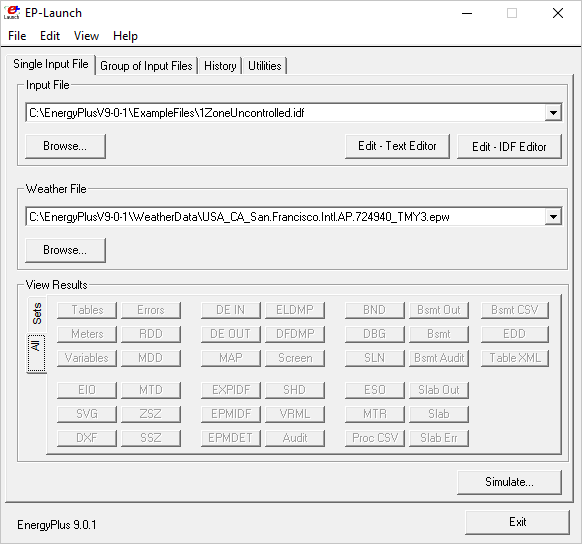
\includegraphics[width=0.9\textwidth, height=0.9\textheight, keepaspectratio=true]{media/eplaunch2.png}
\caption{EP-Launch 2}
\end{figure}


It is a Windows program only. EP-Launch 2 is included in the EnergyPlus
installation package when installing on Windows, so no additional
steps are needed to run it. It is located in the main ``root'' folder
of EnergyPlus, usually, a folder named EnergyPlusVx-x-x, where the
x's are the version number.

In 2018, EP-Launch 3 was developed, and its main screen is shown below:

\begin{figure}[hbtp]
\centering
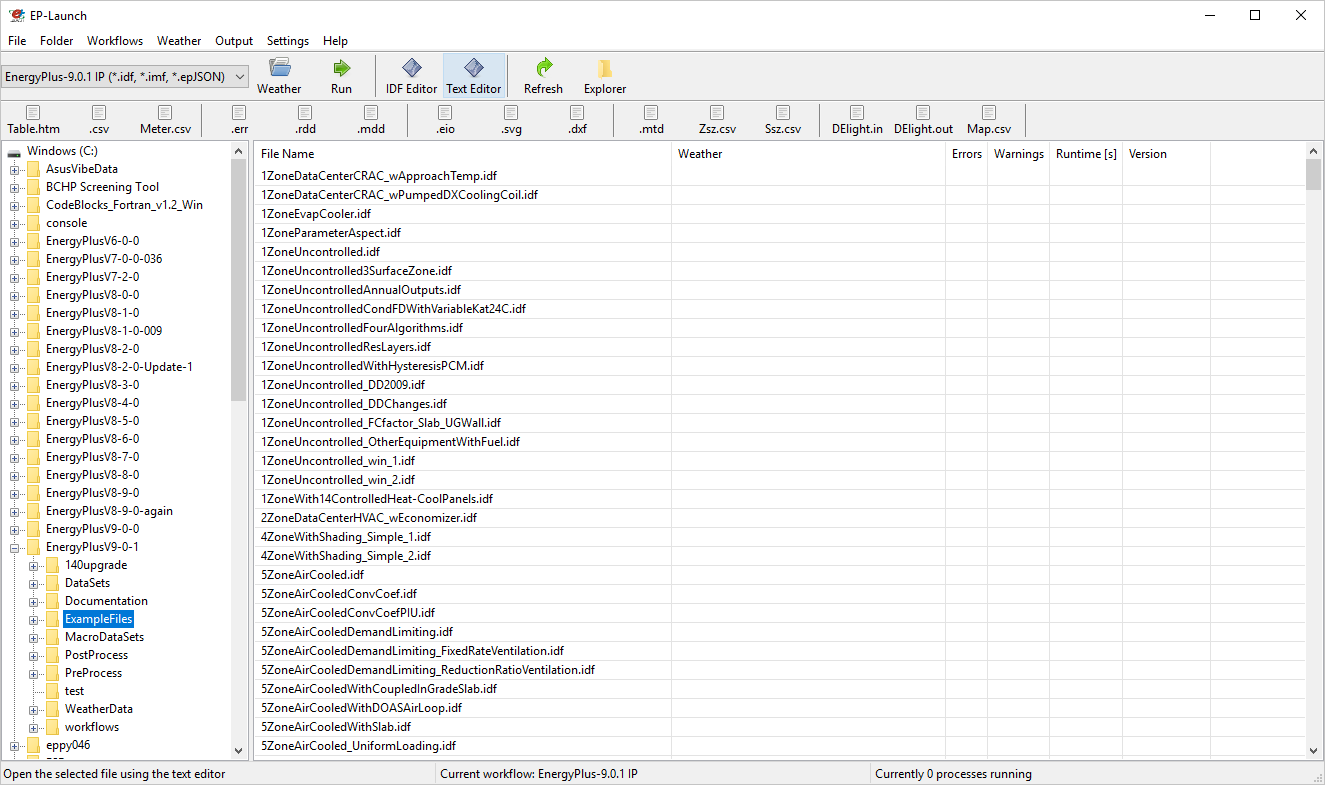
\includegraphics[width=0.9\textwidth, height=0.9\textheight, keepaspectratio=true]{media/eplaunch3.png}
\caption{EP-Launch 3}
\end{figure}


EP-Launch 3 is not part of the EnergyPlus installation package and
needs to be installed separately. It is also open source and is available
from \href{https://github.com/NREL/EP-Launch}{GitHub}, and it is
documented on \href{https://ep-launch.readthedocs.io/en/latest/}{readthedocs}
or in the docs folder on GitHub. EP-Launch 3 works on Windows, MacOS,
and Linux systems and is written in Python.

While both EP-Launch 2 and EP-Launch 3 do many of the same functions,
the interface is quite different. For now, EP-Launch 2 allows groups
of files to be run together and has access to some utilities that
the newer version does not. EP-Launch 3 works across multiple platforms
and is a built from the ground up to be flexible and extensible so
that individuals can make their own workflows that run whatever programs
they need to run.

\section{IDF and JSON syntax}

EnergyPlus has two different input file formats that can be used to
describe the building and system that is simulated. The file extensions
for the two formats are IDF and epJSON. For both input files, the
numeric inputs are in SI units (International System of Units often
called metric units).

\subsection*{IDF}

The legacy file format is a text-based format that describes each
input object in series. Each input object starts with the type of
input object, and each value for each field follows in strict order
separated by commas. The end of the input object is indicated by a
semi-colon. Comments are indicated by an exclamation point ``!''
and anything after this is ignored by EnergyPlus. Commonly, an input
object is spread over many lines in the file with one value for each
field per line. The names of each field are not required but are usually
shown after the value and the comma or semicolon as a special comment
using ``!-'' as an indicator. The input objects can be in any order.
An example of an input object in an IDF file is shown below:
\begin{verbatim}
  Building,
    Simple One Zone,   !- Name
    0,                 !- North Axis {deg}
    Suburbs,           !- Terrain
    0.04,              !- Loads Convergence Tolerance Value
    0.004,             !- Temperature Convergence Tolerance Value {deltaC}
    MinimalShadowing,  !- Solar Distribution
    30,                !- Maximum Number of Warmup Days
    6;                 !- Minimum Number of Warmup Days
\end{verbatim}
The details of this example input object are not important, but the
use of commas, exclamation points, and the closing semi-colon are
important. The IDF format is currently the most commonly used format
throughout the EnergyPlus ecosystem of utilities and GUIs. The list
of possible input objects and fields is documented in the Energy+.idd
file.

A variation on the IDF file format is the IMF file format which includes
macros that can be used for parametric analysis or file management
called EP-Macros. To learn more about macros see the Input Macros
chapter of the AuxiliaryPrograms document.

\subsection*{epJSON}

A new file format based on the industry standard \href{https://www.json.org/}{JSON}
format most often used to transmit data to and from web servers and
web-browser based applications. It is a text-based file format. The
JSON format has wide usage across many industries and is supported
in just about every modern programming language. It is a field-value
style format using brackets and colons to indicate the hierarchy and
commas to separate each field and value pair. The input objects must
appear grouped by the type of input object. The list of possible input
objects and fields is documented in the Energy+.schema.epJSON file
which uses \href{http://json-schema.org/}{json-schema}. The same
input object shown above in IDF format is shown below in epJSON format:
\begin{verbatim}
{
    "Building": {
        "Simple One Zone: {
            "idf_max_extensible_fields": 0,
            "idf_max_fields": 8,
            "idf_order": 3,
            "loads_convergence_tolerance_value": 0.04,
            "maximum_number_of_warmup_days": 30,
            "minimum_number_of_warmup_days": 6,
            "north_axis": 0,
            "solar_distribution": "MinimalShadowing",
            "temperature_convergence_tolerance_value": 0.004,
            "terrain": "Suburbs"
        }
    }
}
\end{verbatim}


\subsection*{Converting between IDF and epJSON}

While the IDF and epJSON file formats are quite different, they contain
the same information, and either may be used. In general, if producing
EnergyPlus input files using a programming language, the epJSON format
might make more sense while, at this point, if producing IDF files
using a GUI, they are likely to use the IDF format. 

EnergyPlus, when
used on the command line, can convert from IDF to epJSON and from
epJSON to IDF using the -c or -{}-convert option.

There is also a separate conversion utility ConvertInputFormat.exe in the root EnergyPlus folder.
It takes the name of an IDF or epJSON input file (with extension) as an argument. For additional options,
type 
\begin{verbatim}
ConvertInputFormat --help.
\end{verbatim}
when in the EnergyPlus folder. This will give the following display
of options:
\begin{verbatim}
Usage: ConvertInputFormat [OPTIONS] input_file [input_file ..]
Options:
  -f, --format ARG                 Output format.
                                   Default means IDF->epJSON or epJSON->IDF
                                   Select one (case insensitive):
                                   default,idf,epjson,json,cbor,msgpack,ubjson,bson
  -h,   -help,   --help, --usage   Display usage instructions.
  -i, --input ARG                  Text file with list of input files to convert
                                   (newline delimited)
  -j ARG                           Number of threads
  -n, --noHVACTemplate             Do not convert HVACTemplate objects.
  -o, --output ARG                 Output directory. Will use input file
                                   location by default.
  -v, --version                    Display version information
Example: ConvertInputFormat in.idf
\end{verbatim}

On Windows, you can also drag a file (IDF or epJSON) onto ConvertInputFormat.exe.
Note that ConvertInputFormat is version-specific and will not convert an epJSON file that is not the same version.

There are three groups of special input objects which are preprocessor commands: GroundHeatTransfer:*,
HVACTemplate:* Parametric:*. ConverInputFormat converts HVACTemplate objects.  EnergyPlus does not convert any of these.


\section{Creating and Editing Input Files}

Since both the IDF and epJSON file formats are text formats, a simple
text editor may be used to edit them. Even if not regularly used,
a good text editor is an important application to have when working
with EnergyPlus. There are many different \href{https://en.wikipedia.org/wiki/Comparison_of_text_editors}{text editors},
and a few have special features related to the IDF format such as
syntax highlighting including \href{https://github.com/bigladder/atom-language-energyplus}{Atom},
\href{https://github.com/jmarrec/notepad}{Notepad++}, and \href{https://energyplushelp.freshdesk.com/}{UltraEdit}.

Another editing choice for IDF file is the IDF Editor which comes
with EnergyPlus in the \textbackslash PreProcess\textbackslash IDFEditor
directory and can be run directly or from EP-Launch. It is a Windows-only
program and was not designed to run on Linux or MacOS. It is specially
designed for editing IDF files and includes many features to simplify
the process. It performs unit conversions so either SI (metric) or
IP (inch-pound) units can be used for editing but the IDF file is
always saved in SI units. It can initialize an input object using
the default values and has indications when values outside the acceptable
range are used. The main screen of the IDF editor is shown below.
Full details of the IDF Editor can be found in the Auxiliary Programs
document under the ``Creating Input Files'' section.

\begin{figure}[hbtp]
\centering
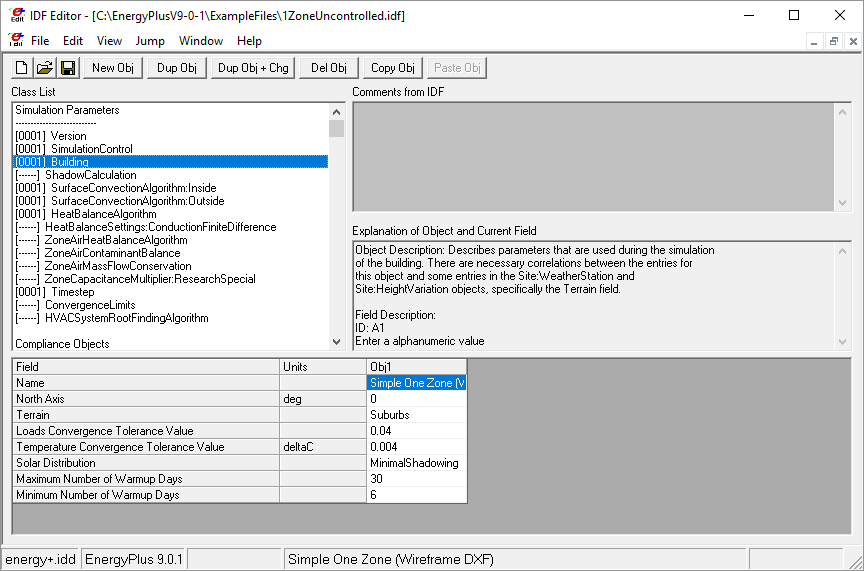
\includegraphics[width=0.9\textwidth, height=0.9\textheight, keepaspectratio=true]{media/idfeditor.png}
\caption{IDF Editor}
\end{figure}

\section{Run-Check-Edit Repeat \label{subsec:Run-Check-Edit-Repeat}}

For most building energy modeling projects, whether assisting in early
design, refining a design, selecting a control method, or calibrating
an existing building, the use of EnergyPlus will be part of a repeating
process. The process will probably be in the form of:
\begin{itemize}
\item Running an EnergyPlus input file
\item Checking error and other output files
\item Fixing the input file
\item Repeat
\end{itemize}
Don't expect that an initial model is ever correct; it is probably
not. Initially, errors are likely to exist. The .ERR file should be
the first file checked each time EnergyPlus is run. The .ERR file
has several levels of messages:
\begin{itemize}
\item Warning
\item Severe
\item Fatal
\end{itemize}
A Fatal error means that EnergyPlus has stopped during the simulation
and the input file needs to be fixed before the simulation can be
run to completion. Fatal errors should be the first thing fixed. Some
Fatal messages reference previous Severe messages so in that case
those should be fixed. Since the entire simulation was not performed,
it is likely that once the fatal errors are fixed that new Severe
and Warning messages will be shown. After all Fatal messages are eliminated,
you should work on Severe messages; they should also be fixed. Finally,
Warning messages should be reviewed. Often Warning messages are informative
and point out unusual configurations, conditions, or choices. If what
is being described by the Warning message is as intended, then the
Warning message can be ignored. More often, the Warning message points
out something that is not as intended and should be fixed or addressed.
Since the .ERR file is a text file; you can usually keep it open in
a text editor program. Many (but not all) text editor programs will
detect that the .ERR file has been updated after each EnergyPlus simulation
and lets you load the most recent version.

The next files to be examined are ones that show output results from
the simulation. Either the tabular output file (usually an HTML file
see Output:Table:SummaryReports and OutputControl:Table:Style) or
CSV file (see Output:Variable and Output:Meter) should be examined
depending on what you want to look at. Upon examination of the output
results, it is very likely that an aspect of the building and its
systems are not behaving as expected. For example, the \textquotedbl Annual
Building Utility Performance Summary\textquotedbl{} report contains
a subtable titled \textquotedbl Comfort and Setpoint Not Met Summary\textquotedbl .
If an annual simulation has 100s or 1000s of hours of setpoint not
met, then the HVAC system is undersized, or the controls are not working
as expected. With an input file representing many thousands of assumptions,
some assumptions made by you or as a default of EnergyPlus are likely
to be incorrect. Revising the EnergyPlus input file to address this
may cause new issues to be shown in the .ERR file so it should \emph{always}
be examined after each change.

To speed the process of running the simulations, you may want only
to run a design day (see SimulationControl and SizingPeriod:DesignDay)
or a subset of the year (see RunPeriod) while developing and debugging
the inputs. This approach speeds up the simulation time itself, and
if used, please remember to recheck the .ERR file when running an
annual simulation for the first time.

\section{Key Concepts}

The following sections highlight some key concepts in EnergyPlus

\subsection*{Everything Included}

One principal that EnergyPlus uses is that (almost) everything is
specified in the input file. This means that instead of referencing
an external library for materials, schedules, equipment performance,
etc., the input objects that fully describe those items should be
included directly in the input file. In addition, each input object
contains a list of values for every field that needs one. The DataSets
folder distributed with EnergyPlus contains these kinds of details
and to use them, the input objects should be copied into the input
file that you are developing. This approach does make the file include
more specification than you might be used to, and typically results
in a large input file, but you will have the assurance of knowing
that all the inputs related to your building are in the input file
you have developed. There are a few exceptions where external data
is referenced such as with Schedule:File input objects.

\subsection*{Wall Thickness}

Exterior and interior walls in real buildings have a thickness as
specified on building plans by detailed cross-sections. For EnergyPlus,
the Construction input object is made up of a list of names for the
Material input objects that make up the wall or roof or floor. Each
material input object has a thickness along with the conductivity,
density, specific heat and other factors. These thicknesses should
match the thicknesses shown in the detailed cross-sections. But when
it comes to specifying the walls themselves in three-dimensional space,
the walls should be entered assuming zero thickness. Once each surface
has been placed, changing the material thickness will have no impact
on zone volume, ceiling height, floor area, shading, or daylighting.
For most modern buildings the choice of where to locate the wall:
inside vs. outside vs. centerline should have little impact on results,
so many modelers just pick one and let the volumes be slightly off.
Using centerlines throughout the model splits the difference. Or some
modelers use outer edges for exterior walls and then use centerlines
for interior walls. If you are modeling a very thick wall, such as
an old stone building, then you also have thermal mass considerations.
If you use the outside edges there will be too much mass, inside will
be too little. Again, centerline will split the difference and will
be very close to the correct amount of thermal mass (possibly losing
some corner mass).

\subsection*{Zones Are Not the Same as Rooms}

A zone, sometimes called a ``thermal zone,'' is a theoretical construct
that usually describes a group of rooms that can be treated as a single
thermal entity. A zone typically includes multiple rooms. Often a
zone can be seen as a group of rooms that share a single thermostat.
In the case of many similar rooms with the same thermal and operating
characteristics, even if many different thermostats are used, they
may still be grouped into a single zone in EnergyPlus.

\subsection*{One Construction Per Surface}

Only one type of construction can be associated with each surface
so if the top half of a wall is made up of a different construction
than the bottom half of the wall, the top half and the bottom half
each need to be represented as separate surfaces.

\subsection*{Available Outputs Created by First Simulation}

Since EnergyPlus creates a custom list of possible output variables
during each simulation, you need to perform a simulation first before
you can see them. To create the list use the Output:VariableDictionary
input object and then check the .RDD and .MDD files that are created.
Select the outputs you want and specify them in the input file.

\subsection*{Always Plan Ahead}

Some preliminary steps will facilitate the construction of your input
file. EnergyPlus requires some information in specified, externally
available formats; other information may require some lead time to
obtain. The following checklist should be completed before you start
to construct your input file.
\begin{itemize}
\item Obtain location and design climate information for the city in which
your building is located. If possible, use one of the weather files
available for your weather period run.
\item Obtain sufficient building construction information to allow specification
of overall building geometry and surface constructions (including
exterior walls, interior walls, partitions, floors, ceilings, roofs,
windows, and doors).
\item Obtain sufficient building use information to allow specification
of the lighting and other equipment (e.g., electric, gas, etc.) and
the number of people in each area of the building.
\item Obtain sufficient building thermostatic control information to allow
specification of the temperature control strategy for each area of
the building.
\item Obtain sufficient HVAC operation information to allow specification
and scheduling of the fan systems.
\item Obtain sufficient central plant information to allow specification
and scheduling of the boilers, chillers and other plant equipment.
\item Obtain utility tariff information when expressing the results as costs.
\item Obtain component cost information when performing life-cycle costs.
\end{itemize}

\section{What Are All These Folders?}

The installation of EnergyPlus includes many different files in different
folders:

\begin{figure}[hbtp]
\centering
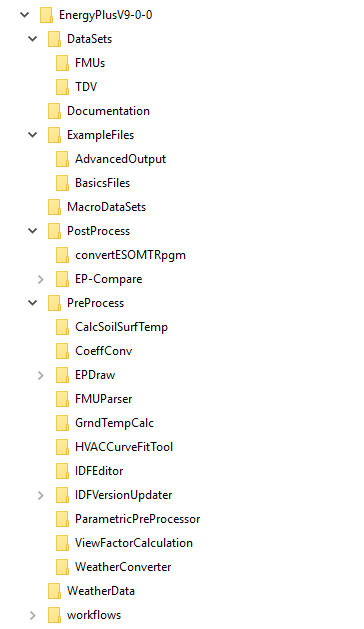
\includegraphics[width=0.9\textwidth, height=0.9\textheight, keepaspectratio=true]{media/energyplusfolder.png}
\caption{EnergyPlus Installation Folders}
\end{figure}

Many of these folders include valuable resources for using and learning
EnergyPlus.
\begin{itemize}
\item The main folder includes the EnergyPlus executable which can be used
on the command line and EP-Launch 2, a program that makes it easier
to use EnergyPlus and the Energy+.IDD that describes each possible
EnergyPlus input object and the default, minimum, maximum, and options
for each field within each input object.
\item The Documentation folder includes this document as well as the InputOutputReference,
EngineeringReference, AuxiliaryPrograms, OutputDetailsAndExamples
which are very important to understand. If you haven't looked through
the documentation yet, take a few minutes and get familiar with it.
\item The DataSets and MacroDataSets folders include files containing libraries
of input objects that may be useful in constructing your own input
files. The ASHRAE\_2005\_HOF\_Materials.idf and WindowConstructs.idf
files, for example, will help with defining walls and windows.
\item The ExampleFiles folder includes a huge number of example files that
are indexed in the two HTML files in that folder or can be searched
through using most text editors.
\item The Preprocess and PostProcess folders include many utilities that
can be used directly or as part of EP-Launch that can aid in the setting
up input files or extracting or converting results. The WeatherData
folder includes a small sample of the many weather files that are
available. For other weather files, please see the previous section
on \ref{subsec:Weather-Files}.
\end{itemize}

\section{What Are All These Output Files?}

When running EnergyPlus using EP-Launch or from the command line,
depending on the options selected, many different output files may
be generated. The file extensions and file suffixes (added to the
original file name prior to the file extension are shown below:
\begin{itemize}
\item ERR -- list of errors and warnings
\item TABLE.HTML, TABLE.TXT, TABLE.TAB, TABLE.CSV, TABLE.XML -- tabulated
report of the bin and monthly data in HTML, space delimited, tab delimited,
comma delimited, or XML format. This is one of the primary otuput
files.
\item CSV, TAB, or TXT -- time series output from the Output:Variable input
object in a comma, tab, or space delimited format (generated by the
ReadVarsESO postprocessor)
\item METER.CSV, METER.TAB, or METER.CSV File -- time series output from
the Output:Meter input object in a comma, tab, or space delimited
format (generated by the ReadVarsESO postprocessor)
\item SQL - sqlite3 output database format
\item EIO -- additional EnergyPlus results
\item RDD -- list of output variables available from the run
\item MDD -- list of output meters available from the run
\item MTD -- list of meter component variables
\item DXF -- drawing file in AutoCAD DXF format
\item AUDIT -- input file echo with input processor errors and warnings
\item BND -- HVAC system node and component connection details
\item DBG -- output from the debug command
\item EDD -- Energy Management System details
\item END - a single line synopsis of the simulation
\item EPMIDF -- clean idf file after EP-Macro processing
\item EPMDET -- EP-Macro detailed output with errors and warnings
\item ESO -- raw Output:Variable output before processing into CSV, TAB,
or TXT files
\item MTR -- raw Output:Meter output before processing into CSV, TAB, or
TXT files
\item SHD -- output related to shading
\item SLN -- output from \textquotedblleft report, surfaces, lines\textquotedblright{}
\item SSZ -- system sizing details in a comma, tab, or space delimited
format
\item ZSZ -- zone sizing details in a comma, tab, or space delimited format
\item MAP -- daylighting illuminance map
\item DFS - daylighting factors report
\item Screen.CSV - window screen transmittance map report
\item RVAUDIT - output from the ReadVarsESO post-processing program
\item SVG - HVAC Diagram related to the arrangement of HVAC components
\item SCI - surface cost information report
\item WRL -- drawing file in VRML (Virtual Reality Markup Language) format
\item Delight IN - DElight input generated from EnergyPlus processed input
\item Delight OUT -- Detailed DElight output
\item Delight ELDMP -- DElight reference point illuminance per time step
\item Delight DFDMP -- DElight warning and error messages
\item EXPIDF -- Expanded IDF when using HVACTemplate input objects
\item Group Error -- combined error files for a group run
\item VCpErr -- Transition program error file
\item Proc.CSV -- Simple statistics generated from CSVProc
\end{itemize}
Most of these output files are documented in the Output Files chapter
of the OutputDetailsAndExamples document.

Don't be intimidated by the long list of files; you can do a lot in
EnergyPlus with just the IDF input file, the TABLE.HTML file, and
the ERR file. The building description, the detecting and solving
of errors, and the most common primary outputs are found between these
three files. Starting with these three files and branching out to
others as needed is a good strategy for using EnergyPlus.

\section{Versions and Updating}

EnergyPlus version updates are released generally twice per year in
March and September. Each version of EnergyPlus is installed to a
unique folder, so it is possible, and recommended, to keep older versions
in place when adding a new one. This is very helpful if you need to
go back and make a change to an older project and don't want to introduce
version-related changes in results. When using the IDF input file
format with EnergyPlus, each release is likely to have small changes
to the file format. Included with EnergyPlus are a number of ways
to update files so that they are compatible with the release. Each
method ultimately uses the TransitionVx-x-x-ToVx-x-x.exe files that
are located in the Preprocess\textbackslash IDFVersionUpdater folder.
The ways to update your IDF files are:
\begin{itemize}
\item IDFVersionUpdater program (shown below) is included in the installation
and works on multiple platforms. It is located in the Preprocess\textbackslash IDFVersionUpdater
folder. It can convert from EnergyPlus 7.2 to the most recent version,
and even older versions can be converted if the proper files are requested
from the \href{https://energyplushelp.freshdesk.com/}{helpdesk}.
It can also update a group of files. It is documented in the Chapter
titled ``Using Older Version Input Files - Transition'' in the AuxiliaryPrograms
document.
\end{itemize}

\begin{figure}[hbtp]
\centering
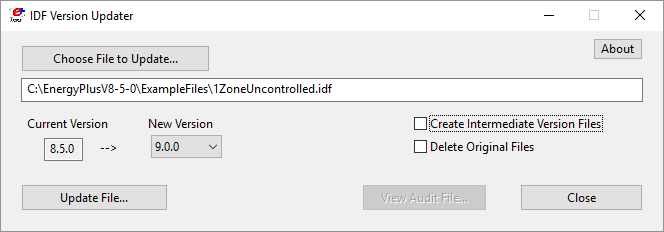
\includegraphics[width=0.9\textwidth, height=0.9\textheight, keepaspectratio=true]{media/IDFVersionUpdater.png}
\caption{IDFVersionUpdater}
\end{figure}

\begin{itemize}
\item EP-Launch 2 - The Windows-only program that comes with the EnergyPlus
installation can update a single file from the just previous version
of EnergyPlus by using the File...Transition command.
\item EP-Launch 3 - The program for Windows, Linux, and MacOS can update
a single file across multiple versions using the Transition workflow.
\item Command line Transition - This allows updating files using the command
line such as the Terminal for MacOS and Linux or the CMD or PowerShell
for Windows. It is documented in the Chapter titled ``Using Older
Version Input Files - Transition'' in the AuxiliaryPrograms document.
\end{itemize}

\section{Errors and How to Fix Them}

As described in the \nameref{subsec:Run-Check-Edit-Repeat} section
dealing with errors described in the ERR file are part of creating
files with EnergyPlus. Resolving errors is something that both new
and very experienced users have to do. Most of the error message itself,
if carefully reviewed will point to the problem. Some error messages
will also reference earlier messages that should also be checked.
A careful review of the ERR file and the input file will often reveal
solutions to the most common errors. Also, see the \nameref{subsec:Getting-Help}
section.

\section{Data Sets}

EnergyPlus uses snippets of IDF files to create the library of data
that may be useful for you. Two folders are created upon installation:
DataSets -- which contains IDF snippets and MacroDataSets -- which
also contain IDF snippets but are in a form such that they can be
easily used with the EPMacro program. Another data set are DDY files
that acompany each EPW weather file. The DDY files include several
varieties of the corresponding design day data for each weather file
location.

\section{Other Useful Utility Programs}

The EnergyPlus install includes a variety of tools to help with various
aspects of converting data or displaying information to help with
using EnergyPlus
\begin{itemize}
\item Coefficient Curve Generation - The CoeffConv and CoeffConv utility
programs can be used to convert DOE-2 temperature dependent curves
(Fahrenheit) to EnergyPlus temperature curves (Celsius). These programs
are described in the Auxiliary Programs document.
\item HVAC Performance Curve Fit Tool - The CurveFitTool.xlsm spreadsheet
generates performance curves for a set of tabular data as typically
supply by manufacturers
\item HVAC-Diagram - Another post-processing program is the HVAC-Diagram
application. It reads one of the EnergyPlus output files (eplusout.bnd)
and produces a Scalable Vector Graphics (SVG) file. Many web browsers
and other drawing programs can open SVG files. This utility runs automatically
with EP-Launch. More information on the HVAC Diagram program is found
in the Auxiliary Programs document.
\item convertESOMTR - This simple post-processing program can be used seamlessly
with EP-Launch to provide IP (inch-pound) unit output files rather
than SI units. This program is described more fully in the Auxiliary
Programs document.
\item WeatherConverter - Used to convert epw to csv format with column headings
to inspection of the data.
\end{itemize}

\chapter{Input Object Groups}

The following sections provide an overview of the input objects based
on groups described in the energy+.idd file and the InputOutputReference.
The sections give you a taste of the capabilities and may help guide
you to further investigation on how to model your building or a specific
energy efficiency measure.

\section{Simulation Parameters}

EnergyPlus includes a group of input objects used to set general parameters
related to how the simulation is performed. Some of these input objects
are controlling different options that are allowed within EnergyPlus
such as the selection of algorithms to use or parameters related to
how an algorithm is used. For a new modeler, these input objects should
be included with their default field values. Later when additional
control is necessary to model a specific type of measure, the field
values can be re-evaluated. The following input object allows you
to control how you want the simulation to be performed. The input
objects should appear in your file and appear in almost all of the
example files:
\begin{itemize}
\item SimulationControl - controls if the simulation is run for the weather
file period and if sizing calculations are performed. You should become
familiar with this input object since you may find it one that you
frequently change during the Run-Check-Edit cycle.
\end{itemize}
Two other input objects should appear in your input file and are included
in almost all example files:
\begin{itemize}
\item Version - indicates what version of EnergyPlus is being used.
\item Building - includes fields for the name of the building, and the angle
of the entire building compared to true north, as well as parameters
related to the simulation that, in general, should be allowed to default.
\end{itemize}
For a new modeler, the following input objects may be omitted. They
can be added later for special cases althought they and appear in
almost all of the example files:
\begin{itemize}
\item Timestep - the number of timesteps each hour and usually set to 6.
\item HeatBalanceAlgorithm - selects the algorithm used for simulating heat
and moisture transfer through the surfaces of the building and usually
set to ConductionTransferFunction.
\item SurfaceConvectionAlgorithm:Inside - selects the algorithm used for
the inside face of the building surfaces and is usually set to TARP.
\item SurfaceConvectionAlgorithm:Outside - selects the algorithm used for
the outside face of the building surfaces between interior and exterior
conditions and is usually set to DOE-2.
\end{itemize}
These input objects and more are further explained in the InputOutputReference
under the heading ``Group-Simulation Parameters.''

\section{Location and Climate}

Many of the fields in the group of input objects related to location,
climate, and the weather file are ones that will be set once for each
specific project.
\begin{itemize}
\item Site:Location - describes the name, latitude, longitude and other
parameters related to the location of the building. When using a weather
file, the values from the weather file will be used instead. Predefined
location objects may be found in the DDY file that accompanies most
epw weather files.
\item SizingPeriod:DesignDay - the high and low temperature and humidities
describing a design day that is used for sizing equipment. Two (or
more) instances of this input object are frequently in a file, one
for heating and one for cooling. The DDY file that comes with the
weather file should include input objects that may be used here.
\item RunPeriod - the start and stop dates of the simulation and often set
to the full year. When debugging a file, a shorter period of time
can be used to speed up the simulation portion of the Run-Check-Edit
cycle.
\item RunPeriodControl:SpecialDays - allows specfication of holidays and
a good example can be seen in 5ZoneCostEst.idf.
\item RunPeriodControl:DaylightSavingTime - allows the specification of
the start and ending period for daylight savings time. This will impact
when schedules operate but please note that output reporting timesteps
are always shown in standard time so schedules will shift an hour
in the output when daylight savings time is active. A good example
can be seen in 5ZoneCostEst.idf.
\item Site:GroundTemperature:BuildingSurface - for one of the ground temperature
algorithms, specifies the average temperature for each month of the
year. This temperature is applied directly to the outside face of
surfaces which use the \textquotedbl Ground\textquotedbl{} outside
boundary conditions. See \textquotedbl Ground Heat Transfer in EnergyPlus\textquotedbl{}
in the Auxiliary Programs document for information about preprocessors.
There are also other more integrated ground heat transfer options,
see Site:GroundDomain:{*} and Foundation:Kiva.
\item Site:WaterMainsTemperature - input for the water temperatures supplied
to the building from underground water mains and should be specified
whenever water heaters are described. A good example can be seen in
5ZoneVAV-ChilledWaterStorage-Mixed.idf. If not specified, some default
assumptions are used for the water temperature supplied to the building.
\end{itemize}



Other input objects in this group can help perform sizing using the
weather file, override the sky temperature, impact the variation of
outdoor conditions with building height (especially important for
tall buildings), work with ground temperatures and ground heat transfer,
override the precipitation in weather files, specify the irrigation
for a green roof, and some advanced properties related to the light
spectrum for window performance. These input objects and more are
further explained in the InputOutputReference under the heading ``Group-Location
and Climate.''

\section{Schedules}

Many aspects of building operation are characterized by timing whether
it is the hours that a building is occupied or when the control systems
are in various modes. Due to this, specifying when something occurs
using the Schedule input objects becomes one of the most common things
to do. It is important to coordinate schedules properly. The operation
of office equipment in a space usually corresponds to occupancy of
that space as does the thermostat set points and fan operation. Because
schedules are such a key input for so many features of a building,
a great deal of flexibility exists in EnergyPlus to specify them.
\begin{itemize}
\item Schedule:Compact - The most commonly used method of specifying schedules
and uses ``Through'' and ``For'' to reduce the amount of input
required.
\item ScheduleTypeLimits - Every schedule input object includes a field
that helps validate the limiting values for the schedule, and this
input object describes the upper and lower limit.
\item Schedule:Constant - If the value of the schedule is the same every
hour of the year, this input object is the easiest way to specify
that value.
\item Schedule:File - At times, data is available from a building being
monitored or for factors that change throughout the year. This input
object allows a column of data from an external file to be referenced
as the values of the schedule. A variation of this input object allows
input specifically for shading.
\end{itemize}

\begin{figure}[hbtp]
\centering
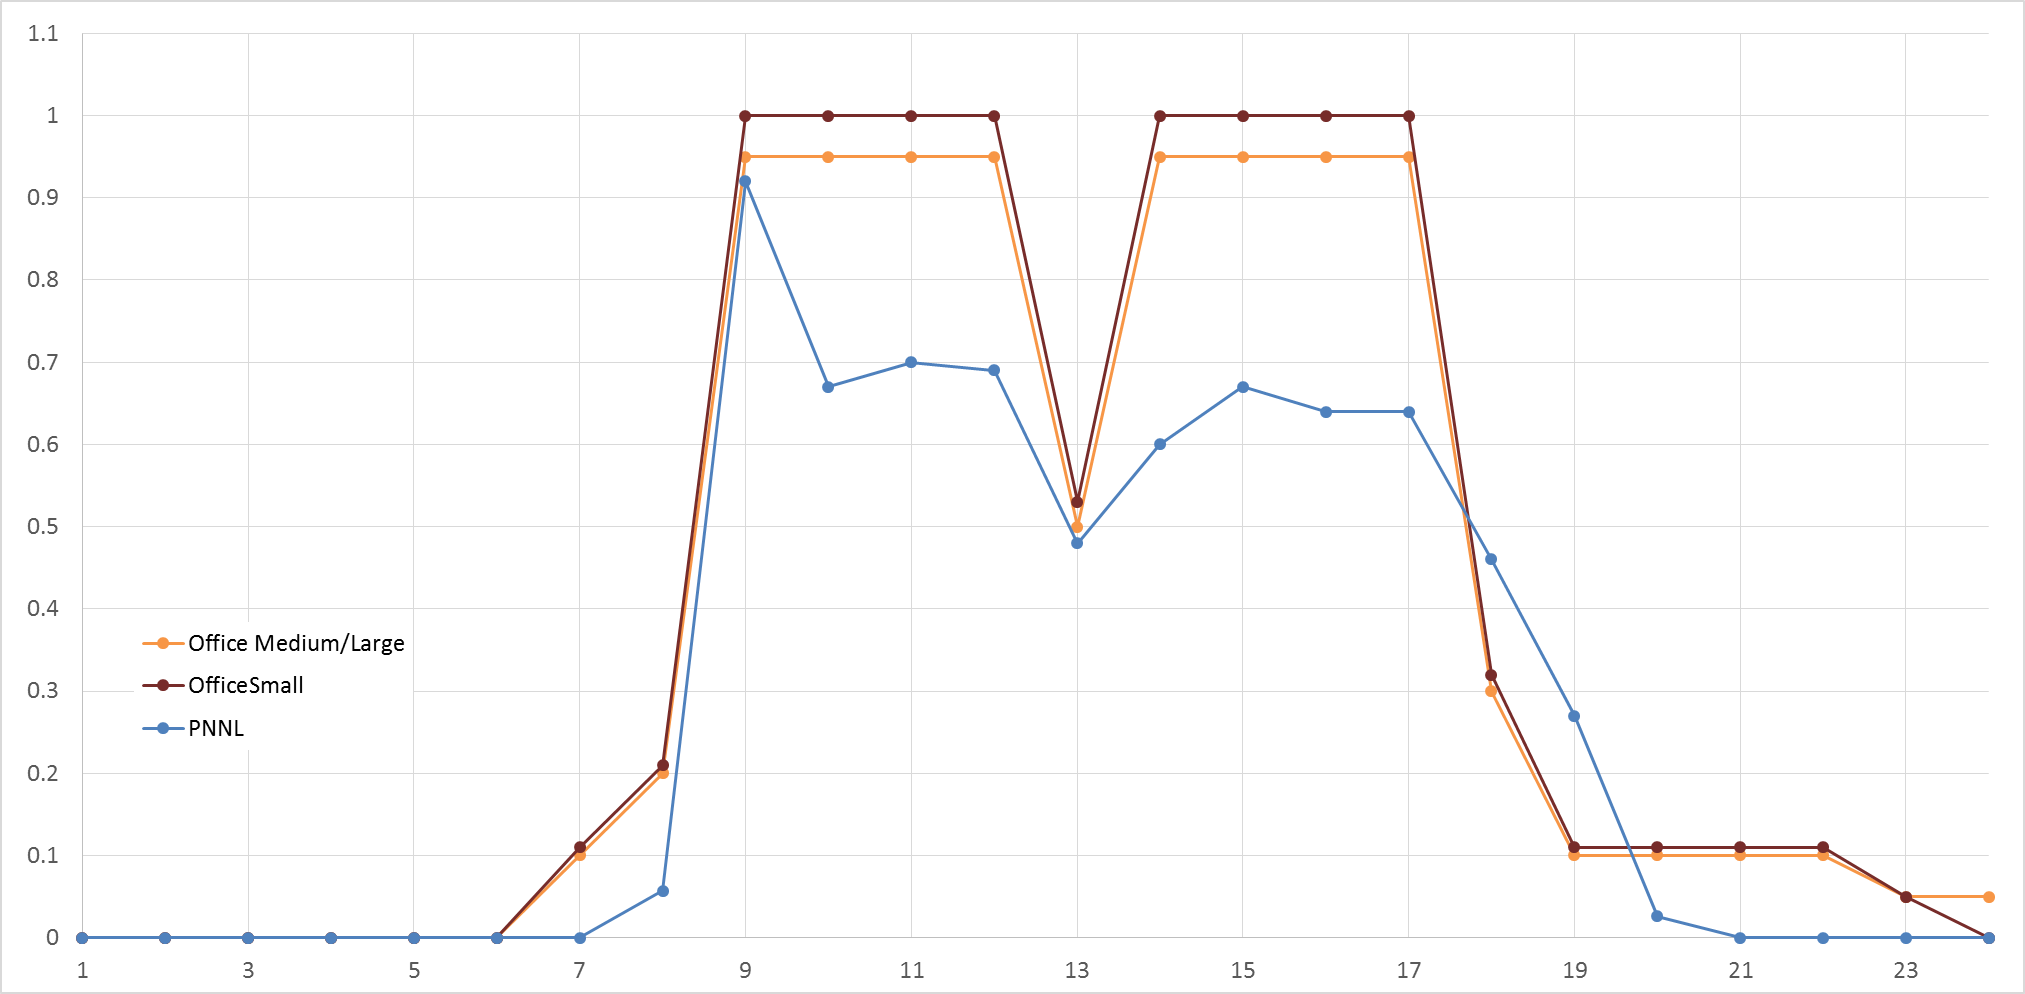
\includegraphics[width=0.9\textwidth, height=0.9\textheight, keepaspectratio=true]{media/officeSchedules.png}
\caption{Various Office Schedules}
\end{figure}


Other input objects in this input group allow specification of schedule
values to be in different formats. These input objects and more are
further explained in the InputOutputReference under the heading ``Group-Schedules.''

\section{Surface Construction Elements}

Specifying the physical properties of the building envelope is something
every building model includes. The input objects in this group allow
the specification of the different layers that make up exterior and
interior walls, roofs, floors, windows, and skylights as well as the
order of the materials in these surfaces. A large number of input
objects appear in this group since there are many special features
that need to be modeled for certain energy efficiency measures. The
following is a list of only the most commonly used input objects.
\begin{itemize}
\item Material - the most common input object to describe the materials
used in opaque constructions in walls, roofs, and floors and includes
inputs for the thickness, conductivity, density, and specific heat
as well as absorptances. See examples in ASHRAE\_2005\_HOF\_Materials.idf
located in the DataSets folder.
\item Material:NoMass - used when the material only has thermal resistance
and little thermal mass such as insulation. It should not be used
to describe materials that do have significant thermal mass.
\item Material:AirGap - used to describe when walls or roofs have an air
gap. Note, this is modeled as a fixed resistance (with no internal
convection or radiant transfer), and it cannot be used for windows.
\item WindowMaterial:Glazing - describes the material used in the glass
(or other transparent material) portion of the fenestration (windows
and skylights). See WindowGlassMaterials.idf in the DataSets folder
for examples.
\item WindowMaterial:Gas - the type of gas used between layers of glass
in windows and skylights has a significant impact on the heat transfer
performance. See WindowGasMaterials.idf in the DataSets folder for
examples.
\item Construction - a list of materials (any from the list above plus others)
in order from the outside to the inside making up the wall, roof,
floor, window or skylight. Every input file will have several of these
input objects. Examples of constructions for walls, roofs, and floors
can be found in ASHRAE\_2005\_HOF\_Materials.idf located in the DataSets
folder while examples for windows and skylights can be found in WindowConstructs.idf
in the same folder.
\item WindowMaterial:SimpleGlazingSystem - the best way to describe a window
is with a construction input object that references WindowMaterial:Glazing
and WindowMaterial:Gas input objects but if all you have is the U-Factor
and Solar Heat Gain Coefficient (SHGC) they can be specified in this
input object.
\end{itemize}

\begin{figure}[hbtp]
\centering
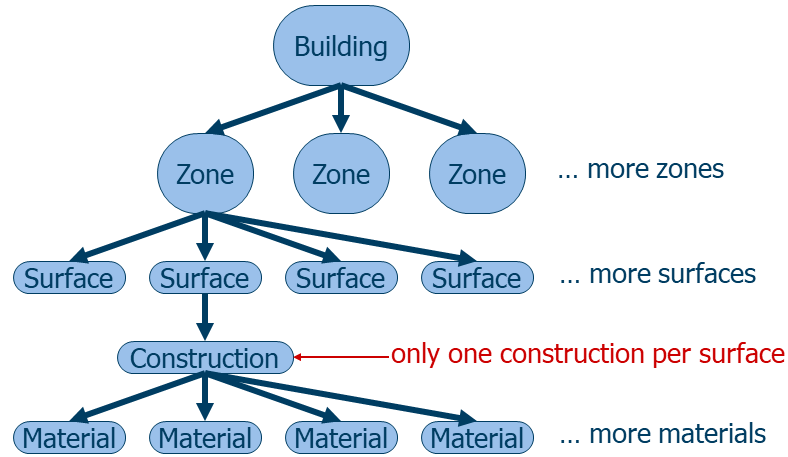
\includegraphics[width=0.9\textwidth, height=0.9\textheight, keepaspectratio=true]{media/EnvelopeHierarchy.png}
\caption{Envelope Component Hierarchy}
\end{figure}

A large variety of input objects in this group are not as commonly
used but are key to modeling specific types of walls and windows so
if what you are trying to model does not fall into the neat categories
for the input objects described so far, there is still a good chance
that EnergyPlus has an input object that will work. These other input
objects include ones for walls and roof that can be used when modeling
combined heat and moisture transfer, modeling materials which undergo
a phase change to store heat in the wall or when the material properties
change with temperature, when the material allows infrared radiation
to flow through it, when modeling green (vegetated) roofs, for simplified
C- or F-factor modeling, or when the wall includes resistance or hydronic
tubing to provide heat. The other input objects to describe windows
and skylights include input objects that can be used to describe thermochromic
and electrochromic glazing, mixtures of gases between layers of glass,
vacuum glazing, movable portions of the window assembly such as shades
and blinds and screens, alternative ways of specifying fenestration
such as equivalent layers or refraction extinction method or ASHWAT
model or from a WINDOW program export/data file or specifying wavelength-by-wavelength
properties.

The input objects described in this section are further explained
in the InputOutputReference under the heading ``Group-Surface Construction
Elements.''

\section{Thermal Zones and Surfaces}

The physical aspects of the building such as the walls, roof, and
windows, is one of the most important and often challenging aspects
of creating a building energy model. In EnergyPlus, the surfaces define
the geometry of each zone and thus for the entire building. For many,
a graphical user interface will be used to help define the geometric
aspects of the building energy model, and many of the input objects
described in this section will be directly created by that interface
program. It is still important to understand some of the details for
these input objects because it is likely that you will be reviewing
them as part of debugging error messages. EnergyPlus uses the three
dimensional position of each corner of a surface to define the position
and orientation of that surface so for a typical rectangular wall
that represents 12 numbers and for a typical building with hundreds
of surfaces that means thousands of numbers are used to define the
geometry of a building so you can see why using an interface is so
common.

EnergyPlus uses a right-hand coordinate system as shown in Figure
X with three dimensions. The X-axis points east, the Y-axis points
north, and the Z-axis points up.

\begin{figure}[hbtp]
\centering
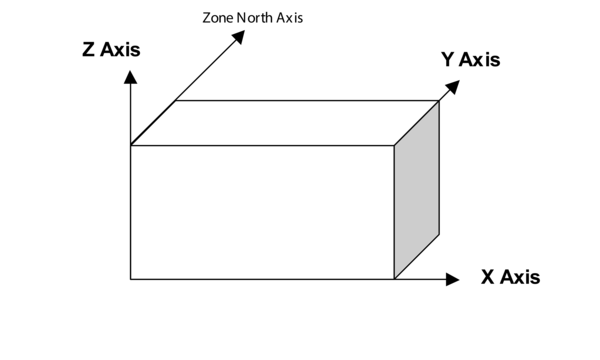
\includegraphics[width=0.9\textwidth, height=0.9\textheight, keepaspectratio=true]{media/coordinatesystem.png}
\caption{EnergyPlus Coordinate System}
\end{figure}

\begin{itemize}
\item Zone - defines the name of the thermal zone as well as the ceiling
height, floor area, and volume. For most zones that are fully enclosed
these three entries can be calculated automatically be EnergyPlus
and do not need to be entered. A zone multiplier allows a single zone
to represent many identical zones (such as all the enclosed offices
on one side of a building). The name of the zone will be referenced
in many places in the input file so it should be clear what it is
describing. When defining a zone, it is important for the entire area
to be thermally similar both in heat being transferred through exterior
walls as well as interior heat gains. But using as few zones as possible
(and thus as few surfaces) also can result in faster simulations,
so there is no reason to slow down the simulation just so two (or
more) essentially identical areas are each simulated. The coordinates
can be just set to zero if the world coordinate system is used (see
GlobalGeometryRules below).
\item BuildingSurface:Detailed - lists the three-dimensional coordinates
that define each corner as well as referencing the zone that the surface
is attached to and the construction of the wall (list of materials).
This input object supports any shape surface with three or more corners
(vertices). In addition, this input object defines what is on the
other side of the surface from the zone, whether that is outside,
another zone in the building, or the ground. Other inputs indicate
if the outside of the surface is exposed to the sun or the wind.
\item FenestrationSurface:Detailed - describes windows, doors, and special
daylighting tubes and it references the wall that it is part of. It
also requires the specification of vertices (usually four but three
is also allowed) to describe the corners of the window or door as
well as the construction which, in this case, is generally the layers
of glass and the gas fill between the layers. It has a field for a
multiplier although usually the multiplier is set to one since the
position of windows matters to many of the algorithms used. In order
to describe the frame of the window and any dividers that it might
have, a separate input object (WindowProperty:FrameAndDivider) may
be included and referenced. A good example file is WindowsTests.idf.
To understand how to model the many options for windows, a section
and a table in the Input Output Reference called ``Window Modeling
Options'' should be examined.
\end{itemize}

\subsection*{Shading Related}

Casting shadows on the building, especially onto windows, can significantly
impact the energy use of a building, and EnergyPlus includes several
input objects to model this effect. The largest impact of shading
surfaces is to reduce solar gain through windows that are shaded.
There are two kinds of shading surfaces in EnergyPlus, detached and
attached. A detached shading surface, such as a tree or neighboring
building, is not connected to the building. An attached shading surface
is typically an overhang or fin that is attached to a particular base
surface of the building, usually a wall; attached shading surfaces
are usually designed to shade specific windows.
\begin{itemize}
\item Shading:Site:Detailed - describes something near but not attached
to the building that casts a shadow on the building such as nearby
buildings or mountains and includes the vertex of one corner as well
as the length and width. For deciduous trees, and other situations
that shading changes over time, the schedule for the transmittance
can vary, otherwise, it should always be set to zero or leave the
schedule name blank.
\item Shading:Zone:Detailed - describes an attachment to the building that
casts a shadow such as an overhang or fin. It also includes a reference
to a transmittance schedule. The wall that the fin or overhang is
attached to is also specified.
\end{itemize}
If using relative coordinates (see GlobalGeometryRules), you may also
want to use the Shading:Building:Detailed input object since it will
``rotate'' with the building. Typically, Shading:Site:Detailed is
used for things that are fixed at the site and don't move with building
rotation. Shading:Building:Detailed is for larger structures like
a parking garage or canopy which aren't associated with a specific
zone but would likely rotate with the building.

\subsection*{Input Object Variations}

EnergyPlus includes a bunch of variations on these basic surface input
objects that map to a closer representation of real surfaces in buildings.
These input objects are effectively just different ways to represent
the same information as the BuildingSurface:Detailed, FenestrationSurface:Detailed,
and Shading:Zone:Detailed input objects. These input objects are seldom
created by graphical user interfaces, so it is unlikely that you will
see them. Some of these input objects also have simpler methods for
specifying geometry, such as using a single vertex, height, width,
tilt, and azimuth or just specifying the fin location relative to
the window edge. The following is a list of these input object variations
for surfaces:
\begin{itemize}
\item Wall:Detailed, Wall:Exterior, Wall:Adiabatic, Wall:Underground, Wall:Interzone
\item RoofCeiling:Detailed, Roof
\item Floor:Detailed, Floor:GroundContact, Floor:Adiabatic, Floor:Interzone
\item Ceiling:Adiabatic, Ceiling:Interzone
\item Window, Window:Interzone
\item Door, GlazedDoor, Door:Interzone, GlazedDoor:Interzone
\item Shading:Site, Shading:Building, Shading:Overhang, Shading:Overhang:Projection,
Shading:Fin, Shading:Fin:Projection
\end{itemize}

\subsection*{Other Related Input Objects}
\begin{itemize}
\item GlobalGeometryRules - A required input object that should be in all
files. It sets the way geometry is specified for all of the surface
input objects. The most common approach is that the order of coordinates
for each surface should start with the upper left corner (when viewed
from ``outside'' the zone with the surface) and that the coordinates
should proceed in a counter-clockwise order. In addition, most common
is to use a world coordinate system where all the vertices are based
on a single coordinate system for the entire building rather than
one that changes relative to each zone. However, if you want to rotate
the building, then you must specify Relative coordinates, and the
zone origins may all remain at (0,0,0).
\item WindowShadingControl - for a window, describes the kind of movable
shading (interior shade, interior blind, between glass shade, exterior
blind, etc..) as well as how it is controlled and the physical material
of the shade or window construction with the shade. Good examples
are in the PurchAirWithDaylightingAndShadeControl.idf file.
\item WindowProperty:FrameAndDivider - defines the frame material around
a window and any dividers between separate lites of the window (see
Figure X). While a window does not necessarily need to define the
frame, it is a more accurate approach since the heat transfer through
the frame usually has significant impacts the overall performance
of a window. Note that the area of the Fenestration:Detailed object
is the glazed area without the frame. The frame extends beyond the
glazed area. See the PurchAirWithDaylighting.idf example file.
\end{itemize}

\begin{figure}[hbtp]
\centering
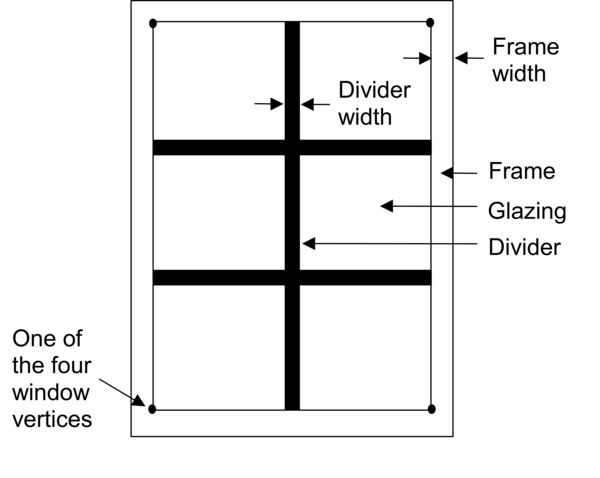
\includegraphics[width=0.9\textwidth, height=0.9\textheight, keepaspectratio=true]{media/window_frame_and_divider.png}
\caption{A window with frame and divider}
\end{figure}

\begin{itemize}
\item WindowProperty:AirflowControl - defines windows that have forced air
flow between the panes of glass, also called heat-extract windows
or climate windows. See the example file AirflowWindowsAndBetweenGlassBlinds.idf.
\item WindowProperty:StormWindow - allows the definition of a movable storm
window that is usually applied to a window in the winter. See the
StormWindow.idf example file.
\item InternalMass - used to define thermal mass that is not described anywhere
else in the model - often used to capture the effect of furnishings
or interior floors that are not being modeled. Used in many example
files including RefBldgLargeOfficeNew2004\_Chicago.idf.
\item ShadingProperty:Reflectance - specifying the reflectance properties
for shading and is only needed if the input object Building specifies
the ``with reflections'' option. See the ReflectiveAdjacentBuilding.idf
example file.
\end{itemize}
Other less common input objects include ZoneList and ZoneGroup that
can be used when doing multi-story simulations and GeometryTransform
which allows a building model to be stretched with just a few inputs.

\section{Internal Gains }

Inside a building, people, appliances, office equipment, lighting,
and other devices produce heat. The combination of all these items
that produce heat within a building are called internal gains and
represents a significant contribution, sometimes the largest contribution,
to the cooling requirements for a building. In addition, they offset
the amount of heat from the HVAC system that is needed at a given
time. Typically, the peak value is entered in the input objects for
this group such as the maximum number of people, the total power of
equipment, or the total lighting power and then a schedule is used
to modify that value each hour of the year. It is just as critical
that the schedule values are realistic for your building as is the
peak value. For almost all buildings, it is rare that the peak occupancy
occurs for more than a few hours per year if at all and this is especially
the case for retail stores, theaters, and sports complexes. Even office
buildings when counting vacations and people out of the building for
meetings will rarely have peak occupancy.

The most common internal gain input objects that are shown in almost
all the example files are:
\begin{itemize}
\item People -- specifies not only the sensible, latent and radiant heat
from people but also includes ways of reporting the comfort of occupants
using a variety of thermal comfort models. The DynamicClothing.idf
example file shows how to use the thermal comfort models.
\item Lights -- describes the heat related to lighting systems.
\item ElectricEquipment -- describes the heat related to electrical appliances,
office equipment, and other heat sources that are powered by electricity.
\item GasEquipment - specifies the heat related to cooking appliances and
other equipment that uses natural gas.
\end{itemize}
Less common internal gains input objects include:
\begin{itemize}
\item OtherEquipment - describes any heat gain or loss (sensible, radiant,
and/or latent) that impacts the space but does not consume utility
energy in the simulation. Typically used to model a process load which
is not to be included in the overall building energy consumption.
\item ElectricEquipment:ITE:AirCooled - see the 1ZoneDataCenterCRAC\_wApproachTemp.idf
example file.
\item SwimmingPool:Indoor - see the 5ZoneSwimmingPool.idf example file.
\end{itemize}
Other
\begin{itemize}
\item ComfortViewFactorAngles -- allows the specification of how different
surfaces impact the thermal comfort calculations for the occupants.
See the PurchAirWithDaylightingAngleFac.idf example file.
\end{itemize}
The Internal Gains group also contains input objects related to zone
contaminant sources and sinks. The input objects include modeling
components that impact contaminant concentrations which are scheduled,
pressure driven, use a cut off model, assume a decaying source, surface
diffusion, or using a deposition velocity model. The input objects
described in this section are further explained in the InputOutputReference
under the heading ``Group-Internal Gains.''

\section{Daylighting }

Reducing the amount of powered lighting that is used when sufficient
natural daylight illuminates the interior building through windows
and skylights is called daylighting. Automatics daylighting control
systems are a very common energy efficiency measure in buildings and
are often required for new building designs depending on the energy
code that applies to the building location. The most common input
objects related to daylighting are:
\begin{itemize}
\item Daylighting:Controls -- specifies the algorithm used for daylighting,
the dimming of lights is continuous or stepped, and how glare calculations
are performed.
\item Daylighting:ReferencePoint -- specifies the location of the sensors
for the daylighting control system.
\end{itemize}
The InputOutputReference includes not only a description of these
input objects but also extra guidance on how they should be applied.
The PurchAirWithDaylighting.idf contains examples of these input objects.

\begin{figure}[hbtp]
\centering

\includegraphics[width=0.9\textwidth, height=0.9\textheight, keepaspectratio=true]{media/DaylightingContinuous.png}
\caption{Daylighting with Continuous Dimming}
\end{figure}


Three different devices can be used with daylighting:
\begin{itemize}
\item DaylightingDevice:Tubular - see the DaylightingDeviceTubular.idf example
file.
\item DaylightingDevice:Shelf - see the DaylightingDeviceShelf.idf example
file.
\item DaylightingDevice:LightWell - see the GeometryTest.idf example file.
\end{itemize}
An input object called Daylighting:DELight:ComplexFenestration is
used with one of the two control methods specified in the Daylighting:Controls
input object when used in conjunction with complex fenestration systems
such as prismatic and holographic glass.

Some flexibility is given to provide extra output related to daylighting
and includes:
\begin{itemize}
\item Output:DaylightFactors -- creates a special report on the factors
used in daylighting. See the ReportDaylightFactors.idf example file.
\item Output:IlluminanceMap -- allows the generation of maps of illuminance
values within each interior zone that uses daylighting controls. The
exact file format can be set using the OutputControl:IlluminanceMap:Style
input object. See the DaylightingDeviceTubular.idf for example of
both input objects.
\end{itemize}
More details of these output options can be found in the OutputDetailsAndExamples
document. The input objects described in this section are further
explained in the InputOutputReference under the heading ``Group-Daylighting.''

\section{Advanced Construction, Surface, Zone Concepts}

The group of input objects contains many special cases for more sophisticated
modeling for constructions, surfaces, and zones. As part of this,
one of the ways to model building foundations called Kiva is described.
See the ZoneCoupledKivaBasement.idf and ZoneCoupledKivaSlab.idf example
files for example of these input objects.
\begin{itemize}
\item Foundation:Kiva - describes the insulation depth and width for interior
and exterior horizontal and vertical insulated foundations as well
as the construction for the wall footing, see Figure X .
\item Foundation:Kiva:Settings - sets the soil conditions and other parameters
related to the Foundation:Kiva input object.
\item SurfaceProperty:ExposedFoundationPerimeter - used to set the portion
of the foundation that is along the exterior perimeter of the building
that undergoes heat transfer with the environment. Edges of underground
surfaces that are fully under the building and not along the perimeter
are not expected to have any heat transfer with the environment.
\end{itemize}

\begin{figure}[hbtp]
\centering
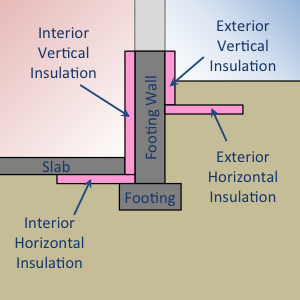
\includegraphics[width=0.9\textwidth, height=0.9\textheight, keepaspectratio=true]{media/kiva-2d-elements.png}
\caption{Structural and insulation components of Foundation:Kiva input objects}
\end{figure}

Input objects of interest in this group not related to Kiva include
\begin{itemize}
\item SurfaceControl:MovableInsulation - allows the modeling of insulation
panels that are removable for walls, floors, and roofs but not windows.
See MovableExtInsulationSimple.idf and MovableIntInsulationLightsLowE.idf
example files.
\item SurfaceProperty:Underwater - allows the outside of the building to
be modeled as underwater and even as moving through the water allowing
EnergyPlus to model vessels. See the VaryingLocationAndOrientation.idf
example file.
\item SurfaceProperty:ExteriorNaturalVentedCavity - provides a method to
include the modeling of baffles in the multi-skin exteriors. See the
HP\_wICSSolarCollector.idf example file.
\end{itemize}
Other input objects in this group set the heat transfer algorithms
for specific surfaces to override the building level heat transfer
algorithm, when other models are used to describe the variation in
temperature on the outside of a surface, override the algorithm used
for modeling convection heat transfer between the air inside or outside
of a zone and the surface, vapor transfer coefficients when using
algorithms that include moisture modeling of surfaces, override the
algorithm that distributes the solar radiation on interior surfaces,
overrides the solar energy absorbed by different layers for complex
windows, a way to override the longwave radiation with other surfaces
in the zone, allows overriding the external environment for a surface
or a zone including solar shading or airspeed or temperature or humidity,
overrides the source term for the heat balance, or overrides the view
factors for a zone. The input objects described in this section are
further explained in the InputOutputReference under the heading ``Group-Advanced
Surface Concepts.''

\section{Exterior Equipment}

While equipment that is outside of a building does not impact the
thermal performance of the building, the accounting of all end-uses
including those outside of the building is important for many compliance
and incentive programs that require building energy modeling. See
the ExteriorLightsAndEq.idf example file for these input objects.
\begin{itemize}
\item Exterior:Lights - describes the external site lighting for the building
grounds, entrances, and facades which are either controlled by a schedule
or when the sun is set.
\item Exterior:FuelEquipment - describes other energy consumption on the
site that is external to the building other than lighting.
\item Exterior:WaterEquipment - describes the flow rate of water use on
the building site outside of the building.
\end{itemize}
The input objects described in this section are further explained
in the InputOutputReference under the heading ``Group-Exterior Energy
Use Equipment.''

\section{Zone Airflow}

The Zone Airflow input object group provides a way to model the airflow
between zones and airflow due to natural ventilation (e.g., open windows)
or mechanically-induced ventilation (e.g., exhaust air fans).
\begin{itemize}
\item ZoneInfiltration:DesignFlowRate - provides a way to describe the air
infiltration into a building through leaks in the envelope including
around windows or the normal operation of doors. The leakage can be
a function of temperature and wind speed and can be expressed as either
a total flow rate, a flow rate per floor area, per wall area, or as
an air change rate. This input object appears in most example files.
\item ZoneInfiltration:EffectiveLeakageArea - similar to the previous input
object but uses a different equation to express the infiltration rate.
The DirectIndirectEvapCoolers.idf file contains an example.
\item ZoneInfiltration:FlowCoefficient - also similar to the ZoneInfiltration:DesignFlowRate
input object but uses yet a different equation.The DirectIndirectEvapCoolers.idf
file contains an example.
\item ZoneVentilation:DesignFlowRate - a method to add outside air to a
zone with similar inputs to the ZoneInfiltration:DesignFlowRate but
this would represent a purposeful introduction of outdoor air into
the space. See the 5ZoneNightVent2.idf example file.
\item ZoneVentilation:WindandStackOpenArea - describes the natural ventilation
driven introduction of outdoor air into the zone using a simpler method
than an AirflowNetwork model. The inputs include the opening area
and effectiveness as well as simple controls based on zone or outdoor
temperature or the difference between the two or wind speed. See the
VentilationSimpleTest.idf file.
\item ZoneMixing, ZoneCrossMixing, and ZoneRefrigerationDoorMixing - these
three input objects provide simplified treatments of air exchange
between zones.
\item ZoneEarthtube - provides a way to model an earth tube which is a way
to draw outdoor into the zone through an underground pipe in order
to cool the air in the summer and heat it in the winter. An example
of this input object is in the EarthTubeSimpleTest.idf file.
\item ZoneCoolTower:Shower - models a passive downdraught evaporative cooling
tower (sometimes also called a shower cooling tower or a wind tower)
using natural ventilation and water evaporation to providing cooling
in typically arid climates. See the CooltowerSimpleTestwithVentilation.idf
for an example of this input object.
\item ZoneThermalChimney - models a passive solar driven thermal chimney
that utilize the buoyancy of air heated by the sun to provide ventilation.
See the file ThermalChimneyTest.idf.
\item ZoneAirBalance:OutdoorAir - calculates the combined outdoor airflow
including the interactions between mechanical ventilation, infiltration,
and duct leakage and is usually applied to residential buildings.
See the SingleFamilyHouse\_TwoSpeed\_ZoneAirBalance.idf file for example.
\end{itemize}
The input objects described in this section are further explained
in the InputOutputReference under the heading ``Group-Airflow.''

\section{HVAC Templates}

New users to EnergyPlus need to learn many things to understand how
to create detailed input objects for modeling an HVAC system. In order
to reduce this initial effort, HVACTemplates were created. Unlike
other input objects, the HVACTemplate input objects are not directly
processed by EnergyPlus; instead, a preprocessor called ExpandObjects
turns these HVACTemplate input objects into the detailed HVAC input
objects. This can be used as a learning tool since you can review
the .expidf file that contains the detailed input objects or it can
be used for long term modeling especially if your focus is not on
HVAC related energy efficiency measures. The primary disadvantage
of using the HVACTemplate input objects is that only a small subset
of possible configurations can be modeled using them; however, the
subset of configurations supported by the HVACTemplate input objects
was carefully chosen to be some of the most common HVAC configurations.
If the HVACTemplate input objects do not support the HVAC configuration
you are considering; you need to model it with the detailed HVAC EnergyPlus
input objects. When using HVACTemplate input objects, no regular EnergyPlus
input objects related to HVAC should be used (see the InputOutputReference
for some exceptions to this). The HVACTemplates can model:
\begin{itemize}
\item Baseboard heating systems with optional hot water boiler
\item Fan coil systems with boilers and chillers
\item Packaged terminal air conditioner (PTAC) system with optional hot
water boiler
\item Packaged terminal air-to-air heat pump (PTHP) systems
\item Water to air heat pumps with boiler and cooling tower
\item Variable refrigerant flow heat pumps (air-to-air)
\item Variable refrigerant flow heat pumps (water-to-air) with boiler and
cooling tower
\item Direct-expansion (DX) cooling, package and split systems
\item Direct-expansion (DX) heat pump systems
\item Packaged variable air volume system using direct-expansion cooling
\item Variable air volume systems with boilers and air-cooled chillers
\item Variable air volume systems with boilers and water-cooled chillers
\item Constant air volume systems with boilers and water-cooled chillers
\item Dual-duct systems (constant or variable air volume) with boilers and
water-cooled chillers
\item Dedicated outdoor air systems (DOAS) combined with zonal template
systems
\end{itemize}
The Input Output Reference includes a list of exactly which input
objects are needed for each of these configurations
\begin{itemize}
\item HVACTemplate:Thermostat - describes the heating and cooling setpoints
for a thermostat. This input object can be referenced by multiple
HVACTemplate:Zone input objects if all the zones have the same setpoints.
\item HVACTemplate:Zone:IdealLoadsAirSystem - provides an idealized system
that supplies air to the zone that meets all loads and uses no energy.
Best used for load calculations.
\item HVACTemplate:Zone:BaseboardHeat - allows the simulation of electric
or hot water thermostatically controlled baseboard heaters.
\item HVACTemplate:Zone:FanCoil - describes a four-pipe fan coil system
with outdoor air intake.
\item HVACTemplate:Zone:PTAC - models a packaged terminal air conditioner
with either electric, gas or hot water heating coil most commonly
used in residential or hotel applications.
\item HVACTemplate:Zone:PTHP - models a packaged terminal heat pump system
most commonly used in residential or hotel applications with either
electric or gas supplementary heater.
\item HVACTemplate:Zone:WaterToAirHeatPump - describes the distributed ``terminal''
portions of a system which uses a medium temperature loop and heat
pumps to provide heating and cooling to the building (also see HVACTemplate:Plant:MixedWaterLoop).
\item HVACTemplate:Zone:VRF - provides input for variable refrigerant flow
terminal units.
\item HVACTemplate:Zone:Unitary - describes a constant volume direct-expansion
system such as a rooftop system or split system. Often paired with
a single HVACTemplate:System:Unitary for a single zone system but
can also be part of a multizone system.
\item HVACTemplate:Zone:VAV - simulates the terminal of a variable air volume
system with reheat.
\item HVACTemplate:Zone:VAV:FanPowered - simulates either a parallel or
series fan power terminal of a variable air volume system.
\item HVACTemplate:Zone:VAV:HeatAndCool - simulates the terminal of a variable
air volume system.
\item HVACTemplate:Zone:ConstantVolume - simulates the terminal of a constant
air volume system.
\item HVACTemplate:Zone:DualDuct - simulates the zone portion of a constant
volume or variable volume dual-duct HVAC system.
\item HVACTemplate:System:VRF - simulates the variable refrigerant flow
system.
\item HVACTemplate:System:Unitary - describes the system portion of a rooftop
or split DX cooling system with electric, gas or hot water heating.
\item HVACTemplate:System:UnitaryHeatPump:AirToAir - details the system
portion of a rooftop or split DX air-to-air heat pump system.
\item HVACTemplate:System:UnitarySystem - models the system portion of a
rooftop or split system and has more flexibility than the previous
two input objects.
\item HVACTemplate:System:VAV - simulates the system portion of a variable
air volume HVAC configuration with chilled water cooling and several
different heating options.
\item HVACTemplate:System:PackagedVAV - describes the system portion of
a packaged direct-expansion (DX) based variable air volume HVAC configuration
with several different heating options.
\item HVACTemplate:System:ConstantVolume - provides input for the system
portion of a constant air volume HVAC configuration with optional
chilled water cooling and several different heating options.
\item HVACTemplate:System:DualDuct - models the system portion of a constant
air volume or variable air volume dual-duct HVAC configuration with
optional chilled water cooling and several different heating options.
\item HVACTemplate:System:DedicatedOutdoorAir - adds a dedicated outdoor
air system (DOAS) which can be used with several of the HVACTemplate:Zone
input objects and contains heating and cooling coils and heat recovery.
\item HVACTemplate:Plant:ChilledWaterLoop - models the chilled water loop
connecting chillers to chilled water coils as well as the condenser
water loop that connects chillers with cooling towers.
\item HVACTemplate:Plant:Chiller - describes a vapor-compression chiller
that provides chilled water to the loop.
\item HVACTemplate:Plant:Tower - models an evaporative cooling tower used
to reject heat from chillers.
\item HVACTemplate:Plant:HotWaterLoop - models the hot water loop connecting
boilers to hot water coils.
\item HVACTemplate:Plant:Boiler - models a boiler that provides hot water
to the loop.
\item HVACTemplate:Plant:MixedWaterLoop - models the medium temperature
loop that serves water-to-air heat pumps as well as cooling towers
and boilers.
\end{itemize}
In addition, this group of input objects includes three plant input
objects that allow the referencing of chillers, towers, and boilers
respectively so that additional details can be described in those
input objects. Example for these are in the ExampleFiles directory
and start with the name HVACTempate. All of these are described in
the \textquotedblleft Input/Output Reference\textquotedblright{} document
under the Group \textquotedblleft HVACTemplates\textquotedblright{}
and please note that this group is described in Chapter 2 while most
of the other groups of input objects are described in Chapter 1. The
expansion process is described in the Auxiliary Programs document
under \textquotedblleft ExpandObjects.\textquotedblright{}

\section{Detailed HVAC}

In buildings, HVAC systems are comprised of components such as fans,
pumps, coils, chillers and boilers connected by ducts or pipes and
controlled by systems using sensors strategically located in the distribution
systems and in the zones. In many respects, EnergyPlus mirrors this
topology by having a large number of components and a means to describe
their connections with one another and their control systems. Every
component in an HVAC system must have an inlet and outlet \textquotedblleft node.\textquotedblright{}
In the actual system, a node might be a point in the system at which
fluid properties can be measured. In an EnergyPlus simulation, the
nodes are points at which fluid properties are evaluated and passed
on to subsequent equipment. Components are linked together to form
various loops within the simulation. Thus, the output node from one
component also serves as the inlet node to the next component. Loops
are constructed combining the components as well as input objects
the describe the arrangement of the components. The figure below shows
a generic example of the loop-node concept. Loop nodes are a key defining
feature in EnergyPlus. As a result, it is recommended that one of
the first steps taken in defining an HVAC system in EnergyPlus be
the definition of a node diagram or map. This is helpful for visualization
of the entire system.

\begin{figure}[hbtp]
\centering
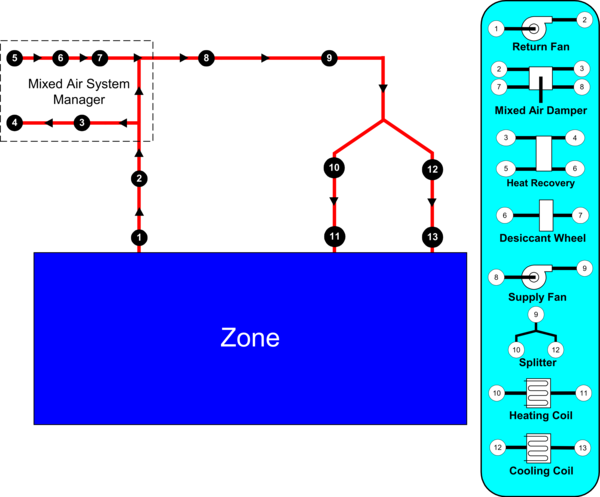
\includegraphics[width=0.9\textwidth, height=0.9\textheight, keepaspectratio=true]{media/NodeDiagram.png}
\caption{Example Node Diagram}
\end{figure}

So that these loops are manageable and more clearly defined both in
the input and in the simulation, four different loop sections can
be defined in an EnergyPlus input file. In general, these four types
are in essence two pairs of loop sections that make up two distinct
types of loops: a zone/air loop and a plant loop.
\begin{itemize}
\item Air Loop Supply Side: The air loop is defined by the section of the
zone/air loop that starts after the zone return streams are combined
and continues on until just before any air stream(s) are branched
off to individual zones. The starting point of the air loop is fairly
straightforward. The ending point is slightly more complex but can
be understood with some examples. For instance, in a terminal reheat
system, the end of the air loop would typically be considered the
node following the cooling coil. In a dual duct system, the air loop
would have two ending points that would correspond to the nodes after
the cooling coil and after the heating coil/humidifier. In most cases,
the air loop has a single starting point and up to two ending points
(for a two-deck system). An outdoor air subsystem can be included
in the supply side for ventilation and relief air.
\item Air Loop Zone Equipment: The zone equipment section of the input file
is defined as more or less the rest of the zone/air loop (outside
air is handled separately as a subset of the air loop). This includes
everything from where the ducts are split to serve various zones up
through where the return ducts from various zones are mixed into a
single return duct. Zone equipment can include dampers and reheat
coils as well as zone-specific conditioning systems such as thermostatic
baseboard or a window air conditioner. Most control issues are typically
dealt with in the zone equipment section of the simulation.
\item Plant Loop Demand Side: One side of the plant is where energy is \textquotedblleft demanded\textquotedblright{}
by various components that make up the air loop or zone equipment.
Typically, this is the water side of equipment such as coils, baseboard,
radiant heating and cooling, etc. In the case of a condenser loop,
energy is typically \textquotedblleft demanded\textquotedblright{}
by a chiller condenser or other water source heat pump. The demand
side of this loop can also include a splitter, a mixer, and a bypass.
\item Plant Loop Supply Side: The other side of the plant loop is where
energy is \textquotedblleft supplied\textquotedblright{} by various
components. The components typically found on the supply side include
pumps, boilers, chillers, purchased heating and cooling, ice storage,
etc. In the case of a condenser, the components would be a cooling
tower, fluid cooler, or ground source heat exchanger, etc. As with
the demand side, this loop can also include a splitter, a mixer, and
a bypass.
\end{itemize}

\begin{figure}[hbtp]
\centering
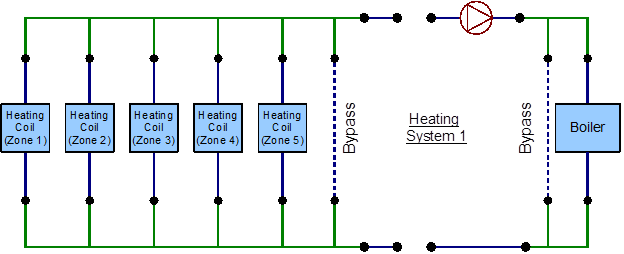
\includegraphics[width=0.9\textwidth, height=0.9\textheight, keepaspectratio=true]{media/HvacHeatLoop.png}
\caption{Detailed HVAC Heat Loop Line Diagram}
\end{figure}

The following is a list of groups of input objects related to specifying
detailed HVAC systems in EnergyPlus related to zone equipment and
secondary systems:
\begin{itemize}
\item HVAC Design Objects - describes input objects related to how EnergyPlus
performs autosizing for air terminals, zone equipment, systems, and
plant components as well as for outdoor air systems.
\item Node-Branch Management - used to describe some of the topological
features of EnergyPlus such as nodes, pipes, and ducts as well as
branches (pieces of loops) and connectors.
\item Air Distribution - describes the arrangement of the components in
an air distribution system includes the outdoor air system, splitters,
mixers, and plenums.
\item Zone HVAC Controls and Thermostats - input objects related to thermostats
and humidistats used to control the conditions in a zone.
\item Zone HVAC Forced Air Units - defines input related to zone forced
air equipment like window air conditioners, packaged terminal air
conditions (PTAC), unit heaters, fan coil systems, and outdoor air
units as well as other related input objects.
\item Zone HVAC Radiative/Convective Units - models baseboard systems, low-
and high-temperature radiant systems, and active portion of ventilated
slabs.
\item Zone HVAC Air Loop Terminal Units - describes air terminals including
constant volume, variable volume, series and parallel powered induction
units, and duel duct terminals.
\item Zone HVAC Equipment Connections - used to describe the HVAC equipment
connections at the zone level.
\item Fans - describes constant volume, variable volume, exhaust fans as
well as more system and component model fans.
\item Coils - contains a long list of input objects to model heating and
cooling water coils; heating and cooling DX coils including two-,
multiple-, and variable-speed units; variable refrigerant coils; fuel
and gas coils; desuperheater coils; air to water heat pump coils;
and other coil input objects.
\item Evaporative Coolers - describes direct and indirect evaporative coolers.
\item Humidifiers and Dehumidifiers - for electric and gas steam humidifiers
as well as desiccant dehumidifiers.
\item Heat Recovery - models for air-to-air flat plate and combined sensible
and latent heat exchangers as well as heat exchangers coupled with
desiccants.
\item Unitary Equipment - describes unitary input objects that are generally
placed in the primary air loop and includes heating only, heating
and cooling, and air-to-air heat pump input objects.
\item Variable Refrigerant Flow Equipment - input objects to describe variable
refrigerant flow (VRF) equipment as well as the controls.
\end{itemize}
The following is a list of control systems in EnergyPlus related to
HVAC
\begin{itemize}
\item Controllers - input objects for simple controllers that look at a
single node and compare it with the setpoint and includes controllers
for water coils, outdoor air, and mechanical ventilation.
\item System Availability Managers - these input objects can take an input
from any node and control whether an entire portion of the HVAC system
is active and can be based on temperature, differential temperature,
schedules, night cycle, and ventilation.
\item Setpoint Managers - these take input from any node or nodes and calculate
a setpoint at another node and include controls for single zone heating,
cooling, or reheat; humidity control; mixed air; warmest or coldest;
and many other scenarios.
\item Plant-Condenser Control - provides control for the plant loop primarily
controlling the operation of the loop and which equipment is available
and includes control based on heating or cooling load and in reference
to outdoor conditions such as dry-bulb or wet-bulb temperature.
\item Plant-Condenser Flow Control - describes the TemperingValve input
object for the special case of flow control with thermal storage systems.
\end{itemize}
The following is a list of input objects related to primary systems
and equipment:
\begin{itemize}
\item Pumps - describes constant speed and variable speed pumps and headered
multiple pump systems.
\item Plant-Condenser Loops - describes the supply and demand side of the
loops the operating temperatures and flow rates.
\item Plant Heating and Cooling Equipment - used to input the central plant
equipment such as steam and hot water boilers; electric, absorption,
engine driven, and turbine chillers; and water-to-water heat pumps;
as well as connections to district heating and cooling sources.
\item Condenser Equipment and Heat Exchangers - describes single-, two,
and variable speed cooling towers; single and two speed evaporative
and non-evaporative fluid coolers; vertical, surface, trench and slinky
ground heat exchangers; and fluid-to-fluid heat exchangers.
\item Non-Zone Equipment - describes the LoadProfile:Plant input object
that allows the load on the plant to be specified by schedule if already
known.
\item User Defined HVAC and Plant Component Models - a group that allows
the user to define custom models for zonal systems, air terminals,
coils, and plant equipment.
\end{itemize}
The input object groups described in this section are further explained
in the InputOutputReference.

\section{Output Reporting}

The primary goal of modeling is seeing the results of the model contained
in the output reporting. EnergyPlus has several different types of
outputs, but initially the most important to understand are the tabular
output reports that summarize the results of the simulation. The Output:Table:SummaryReports
and OutputControl:Table:Style input objects described below are the
only two necessary to start generating the tabular output reports:
\begin{itemize}
\item Output:Table:SummaryReports - allows the specification of different
tabular reports but usually just specifying AllSummary is necessary.
Additional reports can be shown by specifying AllSummaryAndMonthly,
AllSummaryMonthlyAndSizingPeriod.
\item OutputControl:Table:Style - specifying the output format for the tabular
reports which is most commonly HTML but a comma, tab, fixed width,
and XML options are also available. Depending on what is specified
the output reports can have different file extensions and the file
name usually has the word ``Table'' or ``tbl'' in it.
\end{itemize}
You can also create your own custom tabular reports by using one of
the following input objects:
\begin{itemize}
\item Output:Table:TimeBins - shows the amount of time in hours that occurs
in different bins for the single specific output variable or meter
specified
\item Output:Table:Monthly - shows a series of output variables or output
meters on a monthly basis using different aggregation schemes. For
output variables that reoccur for each zone or other input objects,
the monthly report will be repeated for each one.
\item Output:Table:Annual - shows a series of output variables or output
meters on an annual basis using different aggregation schemes. For
output variables that reoccur for each zone or other input objects,
additional rows of results will be displayed.
\item Output:VariableDictionary - provides a list of available output variables
for use with these custom tabular reports as well as the time step
reporting described next. The list of output variables that are available
for specific simulation appear in a file with a .rdd extension, and
the output meters appear in a file with a .mdd extension.
\end{itemize}
When you need to dive deeper into the results for a specific output
variable or output meters, time step outputs allow you to see the
values of an output variable for each timestep or other time periods.
By looking at multiple output variables and seeing how they change
together over time, a deeper understanding of the system and control
operation can be gained.
\begin{itemize}
\item Output:Variable - these input objects are added one for each output
variable desired. Usually, an asterisk is used for the ``key value''
field so that all instances of the output variable are included. The
output shows up in the .eso file which is generally converted to a
.csv file for use with a spreadsheet.
\item Output:Meter and Output:Meter:MeterFileOnly - these input objects
specify the output meters (think of them as very detailed submeters).
The output from these input objects show up in the .mtr file which
is generally converted to a Meter.csv file for use with a spreadsheet.
Also, note that the .mtd file shows the exact relationship between
specific end-use output report variables and each output meter.
\item Output:SQLite - use this input object if you want to output in the
SQLite database format. Not only can the output variables and meters
be in SQLite format but the tabular reports are also included.
\end{itemize}
EnergyPlus also includes a number of special reports that usually
appear in different output files or in the .eio output file
\begin{itemize}
\item Output:Surfaces:List - provides a report on all the surfaces in a
file and the output appears in the .eio and .sln output files.
\item Output:Surfaces:Drawing - provides a DXF drawing that can be opened
in some CAD programs .
\item OutputControl:SurfaceColorScheme - controls the colors used in the
DXF file.
\item Output:Schedules - provides a summary of the schedules in the input
file and appears as part of the file with the .eio extension.
\item Output:Constructions - provides a summary of constructions in the
input file and appears as part of the file with the .eio extension.
\item Output:EnergyManagementSystem - creates a list of detailed output
related to the energy management system in a file with the .edd extension.
\item OutputControl:ReportingTolerances - provides more control over the
amount of time reported for the setpoints not being met.
\item Output:Diagnostics - provides additional detail in the output messages
in the .err file . Normally this extra detail is not shown to reduce
confusion for new users.
\item Output:DebuggingData - provides an additional detailed output related
to HVAC nodes in a file with a .dbg extension.
\end{itemize}
Environmental reporting adds new meters showing the emissions related
to the building and is triggered by the use of the following three
input objects. See the 5ZoneTDV.idf file for examples.
\begin{itemize}
\item Output:EnvironmentalImpactFactors - specifies the frequency of the
output variables related to emissions.
\item EnvironmentalImpactFactors - specifies the efficiency of district
heating and cooling systems as well as the carbon equivalent emission
factors for N20, CH4, and CO2.
\item FuelFactors - for each type of energy resource (electricity, natural
gas, etc..) provides a way to enter factors related to source energy
and emissions of CO2, CO, CH4, NOx, N20, SO2, PM, NH3, NMVOC, Hg,
Pb, and other factors.
\end{itemize}
Other input objects in this group allow the accumulation of metered
results, the combination of output variables or meters to create custom
meters, and a method for preprocessors to include error messages in
the normal error file. Many example files contain some of these input
objects. All of these are described in the \textquotedblleft Input/Output
Reference\textquotedblright{} but note that this group is described
in Chapter 5 ``Input for Output'' and Chapter 7 ``Standard Output
Reports'' while most of the other groups of input objects are described
in Chapter 1. The OutputDetailsAndExamples documentation provides
even more details on the outputs created by each of these input objects.
Several other output related input objects appear in other areas such
as Output:DaylightFactors input object in the Daylighting group.

\section{Economics}

EnergyPlus contains several input objects that allow economic analysis
to be performed. When these input objects are included in the input
file, new tabular output reports are automatically generated. The
input objects used by EnergyPlus for cost estimating calculations
are as follows:
\begin{itemize}
\item ComponentCost:LineItem - provides inputs related to determining the
construction cost and can be associated with several different input
objects and the cost estimate is based on factors such as cost per
area or cost per unit of output capacity. It has not been applied
to all types of input objects so for many scenarios; construction
costing would need to be performed outside of EnergyPlus.
\item ComponentCost:Adjustments - allows the specification of adjustments
including miscellaneous costs per conditioned area, design and engineering
fees, contractor fees, contingency, permitting, bonding, and insurance
as well as commissioning and regional adjustment fees.
\item ComponentCost:Reference - entry of reference building costs so that
the current model can be compared to the reference building.
\end{itemize}
For many building projects, while energy estimates are important,
the computation of estimated utility bills provides an understanding
of how much money is going to be saved to help offset possibly higher
initial costs of a high-performance building. Due to the many different
utility companies and regulatory agencies, the approach used to compute
monthly utility bills has become widely varied and, at times, quite
complicated depending not only on energy and demand but the timing
of each and the relationship between the two. Overall, the goals of
the UtilityCost input objects of EnergyPlus are to make simple tariffs
easy to model and complex tariffs possible to model. The 5ZoneEconomicsTariffAndLifeCycleCosts.idf
example file provides several different example tariffs. The input
objects used by EnergyPlus for the calculation of monthly and annual
utility bills are as follows:
\begin{itemize}
\item UtilityCost:Tariff - sets the parameters for the overall tariff such
as associated output meter, conversion factors, demand computation,
monthly charges, and minimum charges, and schedule names for the time
of use periods, seasons, billing cycle, and real-time pricing.
\item UtilityCost:Qualify - provides a method to qualify if a tariff applies
to the building being modeled since utilities provide limits usually
based on peak demand or energy consumption for each tariff.
\item UtilityCost:Charge:Simple - defines cost per unit value for a charge
based on energy or demand or other charges for a specific season.
The charges are arranged in a hierarchy shown in Figure X Hierarchy
of Economic Charges.
\item UtilityCost:Charge:Block - defines a more complicated but common type
of charge for energy or demand where the costs are defined in the
tariff with blocks of charges (i.e., the first 1000 kWh is one cost
per kWh, the next 5000 kWh is a second cost, and remaining kWh is
a third cost). Like UtilityCost:Charge:Simple, the charges use the
same hierarchy.
\item UtilityCost:Ratchet - some utilities charge not only for the current
month's demand but also compensate for the highest demand in recent
months, and this input object allows the specification of such a structure.
\end{itemize}

\begin{figure}[hbtp]
\centering
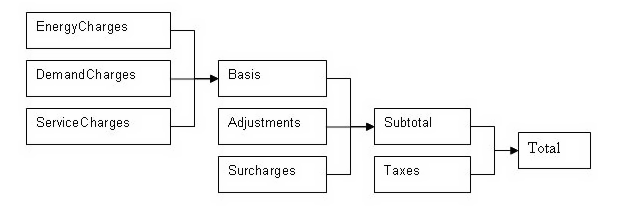
\includegraphics[width=0.9\textwidth, height=0.9\textheight, keepaspectratio=true]{media/tariff-charges.png}
\caption{Hierarchy of Economic Charges}
\end{figure}

The following two input objects are uncommon to use:
\begin{itemize}
\item UtilityCost:Variable - allows the specific specification of a monthly
variable to be used in the calculation of the tariff.
\item UtilityCost:Computation - provides the step-by-step specification
of the steps needed to compute the tariff. The output report tariff
summary includes the default computation steps for the input objects
specified.
\end{itemize}
Life-cycle costing allows the combination of initial and future costs
(typically energy bills) to be understood using a single metric so
that multiple building energy models can be compared even if they
all have different initial and future costs. The input objects used
for performing a life-cycle cost analysis are:
\begin{itemize}
\item LifeCycleCost:Parameters - describes the discount, tax, and inflation
rates, the approach used for inflation and discounting, as well as
the base date and length of the study period and other parameters
related to life-cycle costing.
\item LifeCycleCost:RecurringCosts - used to enter reoccurring costs other
than costs related to energy and water usage since those are included
automatically.
\item LifeCycleCost:NonrecurringCost - used to enter costs that occur only
once during the study period.
\item LifeCycleCost:UsePriceEscalation - specifies the annual escalation
of energy costs in future years and is generally based on government
predictions. The increases in energy costs for future years are assuming
they change differently than inflation. A file that is updated each
year begins with the name LCCusePriceEscalationDataSet is included
in the DataSets directory and is based on supplements to the NIST
135 handbook.
\end{itemize}
Two less commonly used input objects are
\begin{itemize}
\item LifeCycleCost:UseAdjustment - allows manual adjustment of energy or
water costs in future years.
\item CurrencyType - specifies the currency symbol of the monetary unit.
If it is not included a dollar sign '\$' is used in all reports.
\end{itemize}
All of these are described in the \textquotedblleft Input/Output Reference\textquotedblright{}
but note that this group is described in Chapter 3 ``EnergyPlus Economics''
while most of the other groups of input objects are described in Chapter
1. The OutputDetailsAndExamples documentation provides even more details
on the tabular outputs created in the section labeled ``eplustbl.<ext>''.

\section{Other Groups of Input Objects}

The previous sections describe major groups of input objects. This
section briefly covers some of the remaining input object groups.
\begin{itemize}
\item Detailed Ground Heat Transfer - provides an alternative way of describing
ground heat transfer through basement walls and floors and slabs using
input objects that are then processed by the SLAB and BASEMENT programs
and is also documented in AuxiliaryPrograms.
\item Energy Management System (EMS) - a high-level control method that
connects sensors and actuators with a simple control programming language
and is also documented in the EMSApplicationGuide.
\item External Interface - allows the connection of EnergyPlus using co-simulation
by the import of Functional Mockup Units (FMUs) and is also documented
in the ExternalInterfacesApplicationGuide.
\item Operational Faults - provides for the modeling of operation problems
in sensors, controllers, meters, equipment, and systems and is commonly
used with existing buildings.
\item General Data Entry - contains the Matrix:TwoDimension input object
used with the Construction:ComplexFenestrationState input object.
\item Performance Curves - allows the specification of polynomial curves
used to characterize the performance of HVAC equipment.
\item Performance Tables - allows the specification of tables used to characterize
the performance of HVAC equipment.
\item Fluid Properties - describes the detailed properties of refrigerants
and glycols.
\item Demand Limiting Controls - provides a way of implementing management
of the systems of the building to regulate the peak demand.
\item Natural Ventilation and Duct Leakage - provides a way to model multizone
airflows driven by wind and forced air systems (shown under Group-Airflow
Network in the InputOutputReference).
\item Room Air Models - allows the description of non-uniform room air temperatures
(not fully mixed).
\item Compliance Objects - provides an input object that allows rotation
of the building when used for compliance purposes.
\item Parametrics - allows for simple parametric cases to be defined within
an input file using input objects. Makes use of the ParametricPreprocessor
as described in the AuxiliaryPrograms document.
\item Refrigeration - describes supermarket and warehouse refrigeration
systems.
\item Electric Load Center-Generator Specifications - allows the specification
of fuel and photovoltaic generators and controls on when they should
be used to provide power to the facility.
\item Water Systems - contains input objects to describe the use of water
in the building including from wells, rain, and storage.
\item Solar Collectors - describes various systems that convert solar energy
into thermal energy including those that are integrated with photovoltaic
systems.
\item Water Heaters and Thermal Storage - describes systems that provide
water heating and storage as well as ice and chilled water storage.
\end{itemize}
